\chapter{Analýza a návrh řešení}
\label{chap:analyza}

Pro účely real-time renderování grafiky se běžně využívá metod přímé rasterizace\footnote{V současnosti existují i přístupy využívající technik sledování paprsku (ray tracing) pracující v real-time. Pro některé scény mohou být dokonce efektivnější, nicméně jejich implementace na GPU je obtížnější a standardem v oboru real-time počítačové grafiky je stále přímá rasterizace.}. Existuje několik grafických API, které pro tyto účely využívají grafický hardware a dosahují tak pozoruhodného výkonu. Dvěmi nejběžnějšími API pro práci s 3D grafikou jsou v současnosti DirectX a OpenGL. Technologie DirectX je standardem v oblasti počítačových her a je vázaná na platformu Windows. Naproti tomu OpenGL je platformově nezávislá knihovna dosahující srovnatelných výsledků. Obě technologie pak pracují s GPU a využívají tzv. grafickou pipeline poskytovanou hardwarem.
Z průzkumu stávajících řešení vyplývá, že realistického real-time zobrazení na úrovni listů lze v současné době dosáhnout efektivně využitím geometrické ploškové reprezentace. Pro její zpracování je optimalizován grafický hardware a takto popsané stromy lze i věrně rozpohybovat. Jeví se proto jako výhodné, využít ji pro zobrazování instancí stromů s nejvyšším stupňěm detailu. Postup zpracování grafických primitiv na GPU je znázorněn na obrázku (~\ref{fig:gpupipeline}).

\begin{figure}[!hbt]
\begin{center}
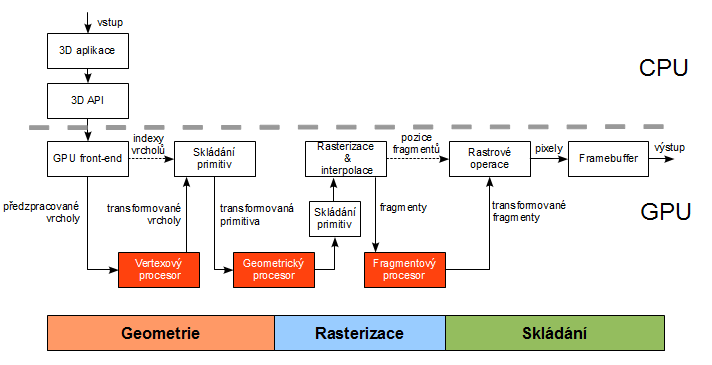
\includegraphics[width=0.85\textwidth]{./figures/GPUpipeline.png}
\end{center}
\caption[Grafická pipeline]%
{Grafická pipeline. Oranžově zvýrazněné bloky lze přeprogramovat a využít k vlastnímu zpracování grafiky.
\label{fig:gpupipeline}
}
\end{figure}

Nížší úrovně následně vytvořeného LOD-systému budou z této nejpodrobnější úrovně odvozeny a abstrahovány. Pro věrné zobrazení stromu pohybujícího se vlivem větru je třeba poznat, jak na vítr strom reaguje. Teoretické základy takové animace rozebere právě následující sekce.

%%%%%%%%%%%%%%%%%%%%%%%%%%%%%%%%%%%%%%%%%%%%%%%%%%%%%%%%%%%
\section{Animace geometrického 3D modelu}
\label{sec-animation3D}

Jelikož je model tvořen množinou trojúhelníků a ty mají přímou vazbu na části stromu (list, konkrétní větev), lze tedy vhodnou změnou jejich polohy animovat celý strom. Požadavek na provádění animace v reálném čase prakticky implikuje i potřebu využití GPU pro tyto účely. Grafická primitiva tvořící model jsou zpracovávána na GPU po vrcholech (vertexech) ve vertex shaderu, který může měnit jejich pozici. 
Metoda, jíž lze s výhodou použít, je popsaná v již zmíněném článku \cite{Habel_09_PGT} a využívá myšlenky tzv. hierarchical vertex displacement. Důležitý je zde fakt, že skutečné větve stromů tvoří hierarchickou strukturu a transformaci nadřazené větve v bodě napojení přejímá celá skupina větví podřízených, což tvoří netriviální řetěz transformací. Tato skutečnost svazuje do určité míry výpočet polohy nadřazené a z ní vycházející větve. Poskytneme-li však vhodná data každému vrcholu, může být celý řetěz transformací určen právě pro každý jednotlivý vrchol korektně a výpočet animace se tak provádí na GPU ve vetrex shaderu.

%%%%%%%%%%%%%%%%%%%%%%%%%%%%%%%%%%%%%%%%%%%%%%%%%%%%%%%%%%%%%
\subsection{Deformace větví}
\label{sec-branchDeformation}

Deformace tak složitých objektů, jako jsou stromy, vlivem větru je komplexní fyzikální problém. Na jeho složitosti mají zásadní vliv zejména dva faktory – netriviální mechanické vazby jednotlivých větví a turbulentní proudění vzduchu, které způsobuje výsledný pohyb. Oba faktory se navíc vzájemně ovlivňují. Aktuální pozice dané větve ovlivňuje proudění v okolí a opačně. I pokud bychom nahradili turbulentní proudění laminárním, jde o složitý problém. Samotný ohyb jedné větve lze sice relativně dobře popsat, ovšem musíme uvažovat, že každá větev je napojena na další a tím ovlivňuje její ohyb. Síly působící na listy i větve samotné vlivem proudění vzduchu se přenáší hierarchií větví až ke kmeni. Jde vlastně o složitý problém inverzní kinematiky, který pro takto složité struktury zatím nelze běžně řešit v real-time. 
\begin{figure}[!hbt]
\begin{center}
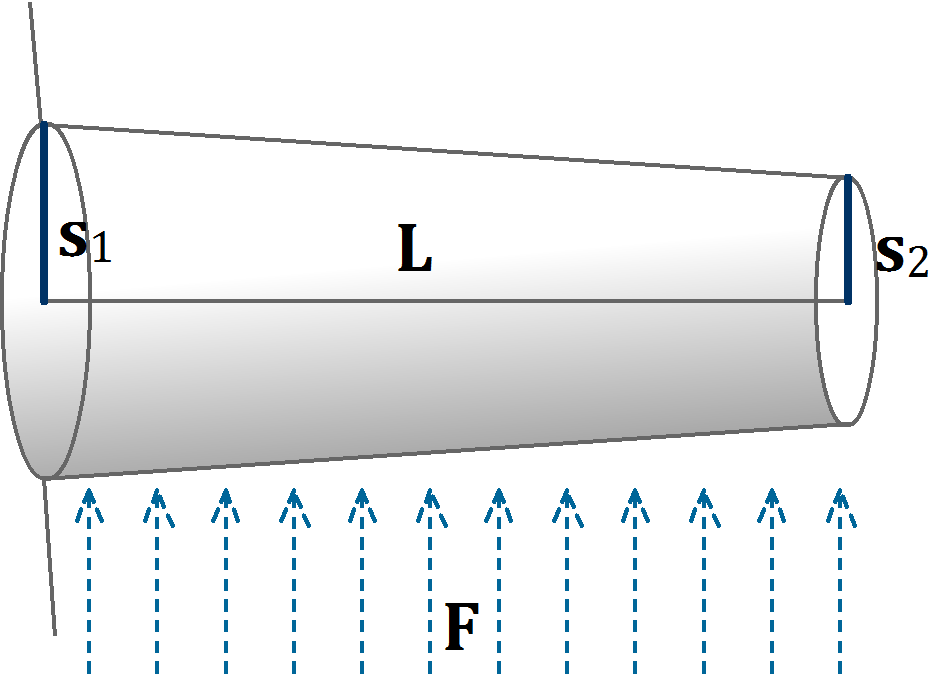
\includegraphics[width=0.25\textwidth]{./figures/branchBeamModel.png}
\end{center}
\caption{Fyzikální model pružného prutu (větve).
\label{fig:branchBeamModel}
}
\end{figure}

Aby bylo možné dosáhnout dostatečného zobrazovacího výkonu, je nutné rezignovat na úplnou fyzikální korektnost výpočtů deformace. Tuto relaxaci problému si naštěstí můžeme dovolit, neboť systém nemá ambice být fyzikálním simulátorem a předpokládá se, že uživatel se spokojí s výsledkem, který nebude výrazně porušovat jeho představu o deformaci vegetace.
Aby byla animace pohybu větví co nejvěrnější, je využita deformace vycházející z Euler-Bernoulliho popisu ohybu prutu. Větev je aproximována komolým kuželem s definovanou délkou $L$ a poloměry na počátku $s_1$ a na konci $s_2$. Tuhost tělesa je závislá pouze na průřezu. A na těleso působí kolmo síla $\vec{F}$ (viz obr. ~\ref{fig:branchBeamModel} ).

Euler-Bernoulliho rovnice pak popisuje ohyb takového tělesa:

\begin{equation}
\frac{\mathrm{d}^2 }{\mathrm{d} x^2}(EI(x)\frac{\mathrm{d}^2 \dot{u} (x))}{\mathrm{d} x^2} ) = F
\end{equation}

V tomto vztahu představuje $I$ plošný moment setrvačnosti a $E$ je modul pružnosti, který je uvažován jako konstantní. Okrajové podmínky na počátku (pevný konec) jsou :

\begin{equation}
\begin{array}{cc}
\dot{u} \mid _{x=0} = 0 & \frac{\mathrm{d} \dot{u} }{\mathrm{d} x}\mid _{x=0} = 0 \\
\end{array}
\end{equation}

a na konci jsou:

\begin{equation}
\begin{array}{cc}
\frac{\mathrm{d}^2 \dot{u} }{\mathrm{d} x^2} \mid _{x=L} = 0 & \frac{\mathrm{d}^3 \dot{u} }{\mathrm{d} x^3}\mid _{x=L} = 0 \\
\end{array}
\end{equation}

Provedeme zjednodušení, kde normalizujeme rozměry délkou $L$ a zavedeme konstantu $\alpha$, která udává poměr velikosti poloměrů na začátku a na konci prutu, také poupravíme modul pružnosti $E$ :

\begin{equation}
\begin{array}{ccc}
r_{1,2} = \frac{s_{1,2}}{L} &\alpha = \frac{r_2}{r_1} & {E}'= EL\\
\end{array}
\end{equation}

Plošný moment setrvačnosti pro kruhový průřez poloměru $r$ je dán vztahem:
\begin{equation}
I = \frac{\pi r^4}{4}
\end{equation}

Protože uvažujeme, že poloměr prutu se mění lineárně v podélné ose prutu, plošný moment setrvačnosti $I$ se mění takto:
\begin{equation}
I(x) = \frac{\pi r_{1}^4((\alpha -1)x + 1)^4}{4}
\end{equation}

Euler-Bernoulliho rovnice pro zmíněné okrajové podmínky a měnící se plošný moment setrvačnosti $I(x)$ má netriviální řešení
\begin{multline}
\dot{u}(x)=\frac{{E}'F}{r_{1}^4}(x(\alpha-1)(6+x(\alpha-1)(2x(\alpha-1)(3+(\alpha-3)\alpha)+3(4+(\alpha-2)\alpha)))\\
 - 6 (1+x(\alpha-1))^2 \log (1+x(\alpha-1))) \cdot  (3\pi(1+x(\alpha-1))^2(\alpha-1)^4)^{-1}
\end{multline}

\pagebreak
Tento vztah je však příliš složitý pro efektivní a rychlé vyhodnocení. Důležitý je postřeh, že funkce $\dot{u}$ je lineárně závislá na velikosti síly $|\vec{F}|$. Fitováním nalezneme funkci s velmi podobným průběhem ve tvaru:

\begin{equation}
\label{eq:bendFunction}\mathbf{
u(x) = c_2 x^2 + c_4 x^4}
\end{equation}

Koeficienty $c_2$ a $c_4$ reprezentují hodnoty ${E}'$, $\alpha$ a $r_1$. Ohybová funkce $u(x)$ tedy určuje, jaká bude výchylka bodu kolmo na podélnou osu prutu ve vzdálenosti $x$ od počátku větve (předchozí normování zajišťuje, že větev zde má vždy jednotkovou délku). Vytváří tak ohybovou křivku. Derivaci ohybové funkce v bodě $x$ označíme ${u}'(x)$.

Ovšem bod na ohýbaném prutu se ve skutečnosti nepohybuje po přímce kolmé k podélné ose, nýbrž opisuje složitou křivku danou i faktem, že délka prutu se při deformaci nemění. Pokud by však byl použit přímo tento vztah pro deformaci, docházelo by k viditelnému efektu prodlužování prutu (větve) s většími výchylkami. Z toho důvodu je nutné zavést určitou korekci, jež bude ve výsledku zachovávat stejnou délku prutu pro libovolnou výchylku. Pokud bychom chtěli zachovat přesnou délku, bylo by nutné vždy vyřešit křivkový integrál, což je příliš časově náročné, a proto se spokojíme s nepřesnou, avšak dostačující a především rychlou metodou.
Vyjdeme z předpokladu, že pro korekci délky stačí posunout bod $P_0$ o určitou vzdálenost $d$ po přímce tečné v tomto bodě s ohybovou křivkou. Získáme tak výsledný bod $P$. 

\begin{figure}[!hbt]
\begin{center}
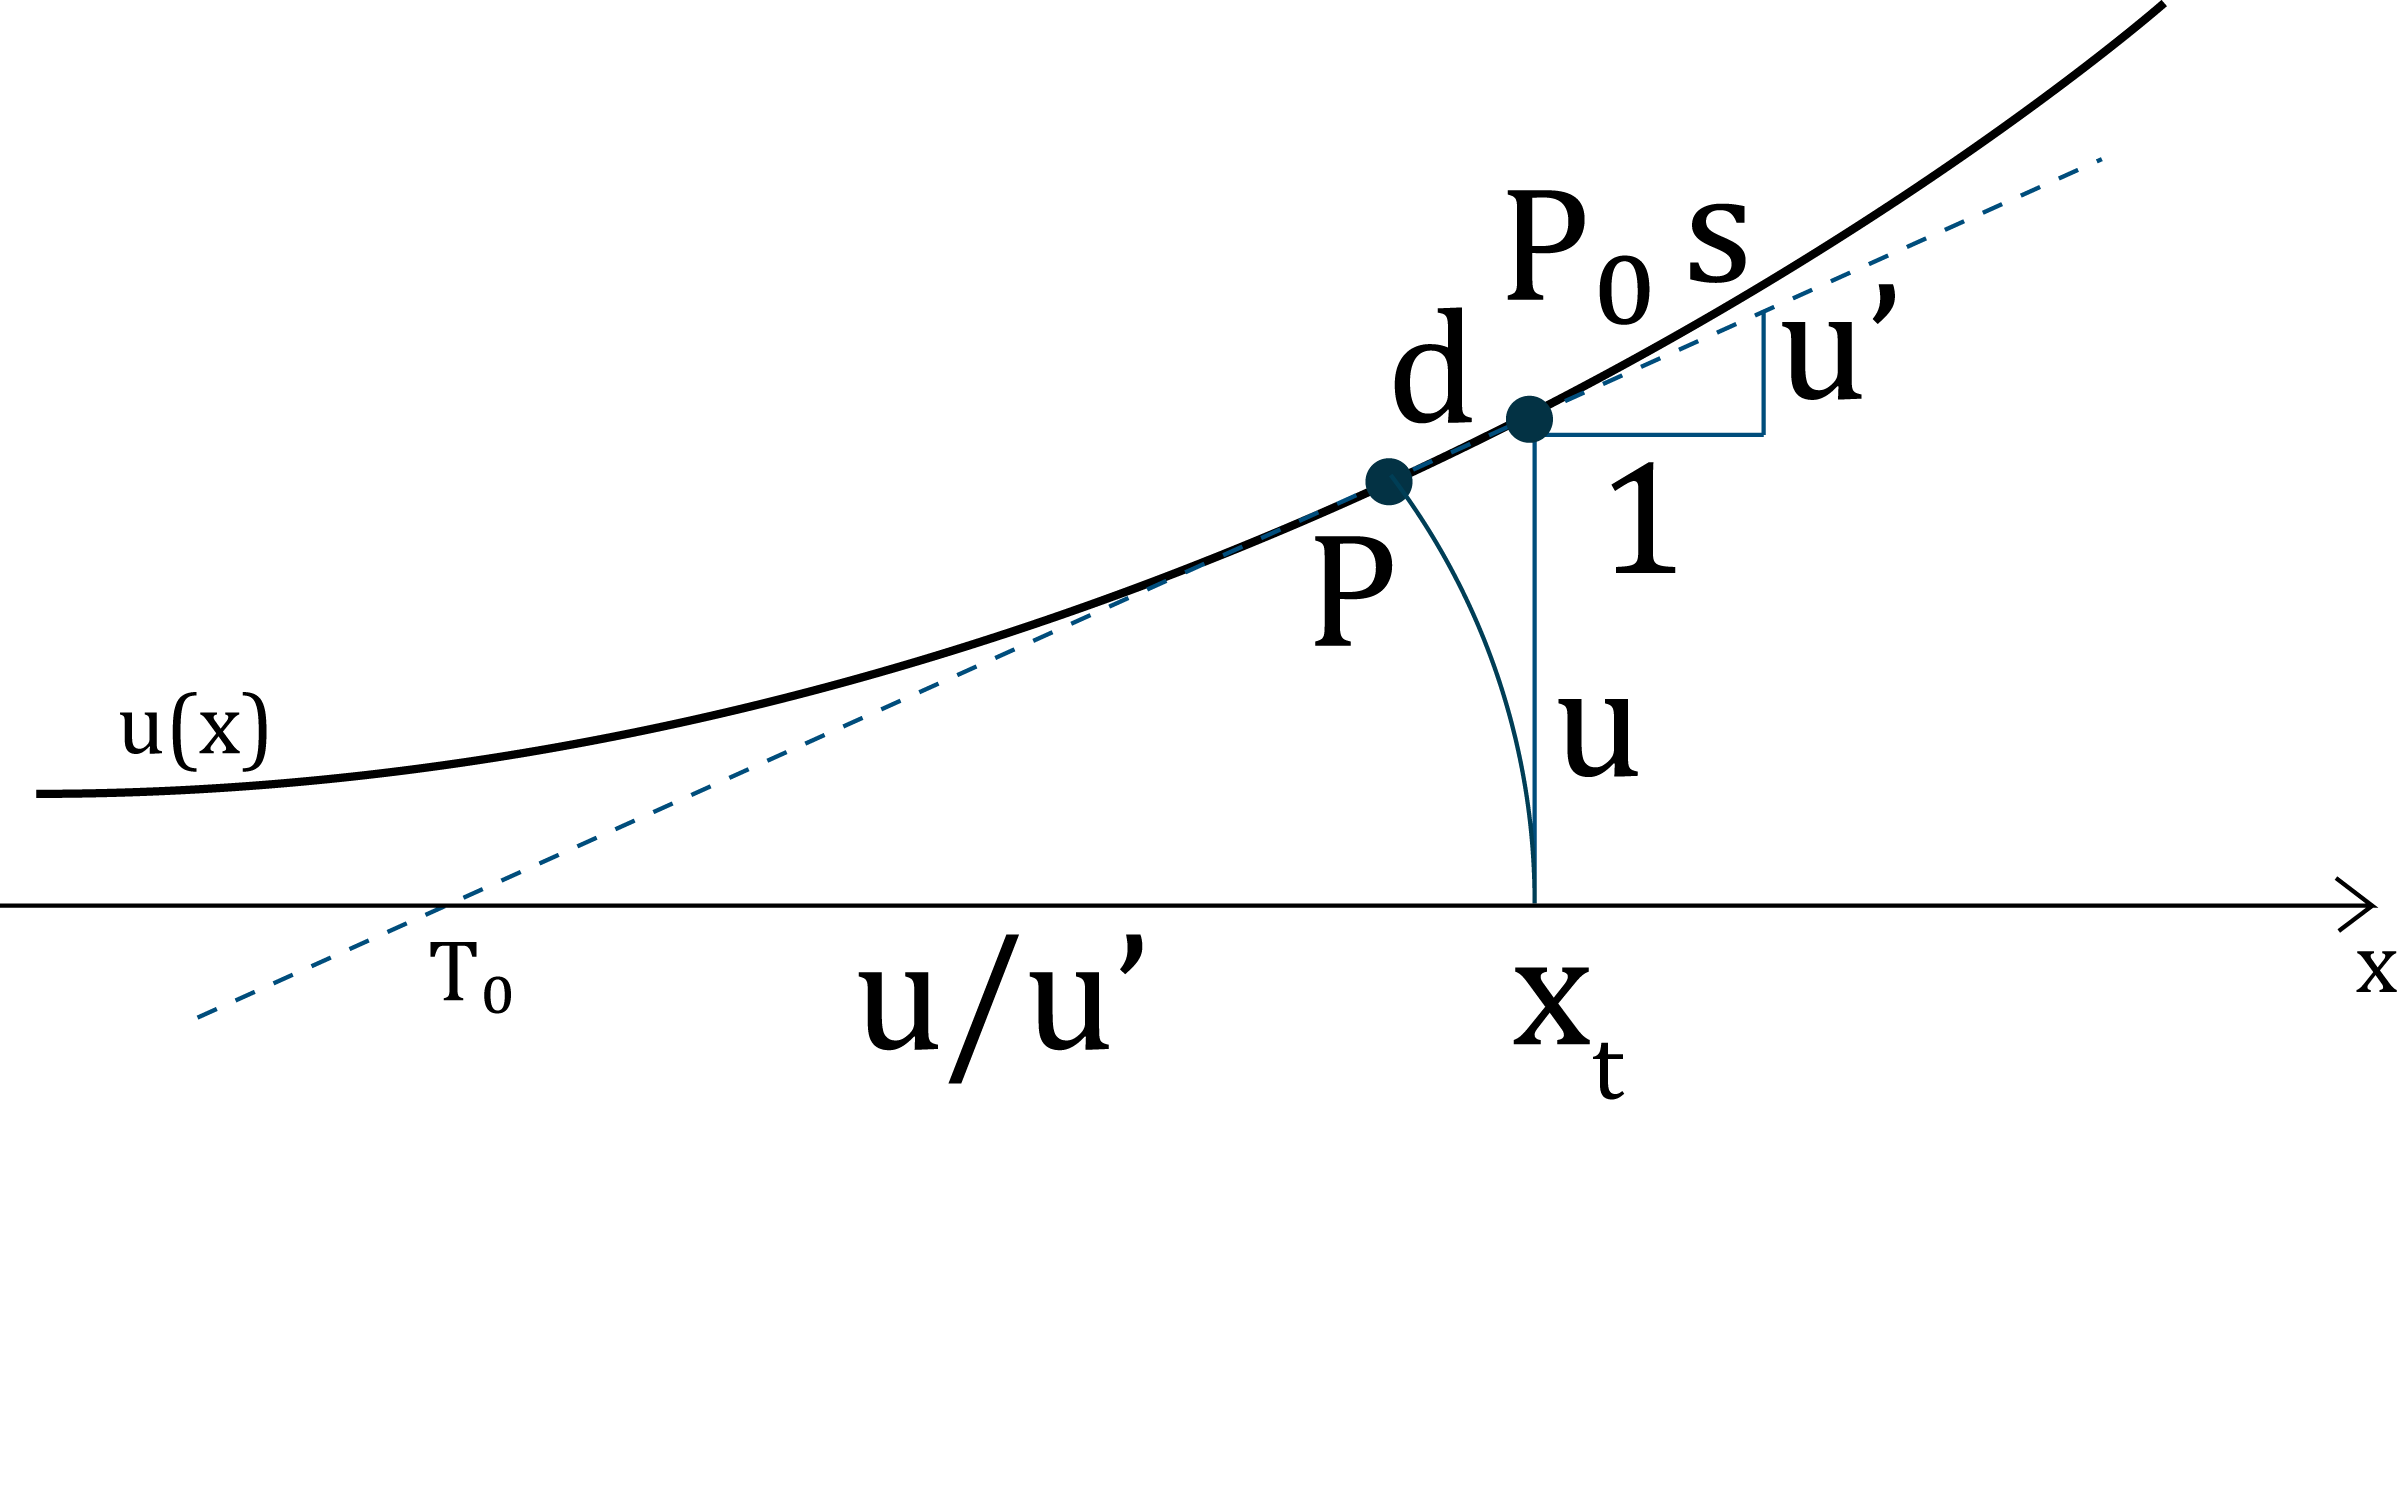
\includegraphics[width=0.5\textwidth]{./figures/lengthCorrection3.png}
\end{center}
\caption[Korekce délky ohybové funkce]%
{Korekce délky ohybové funkce $u(x)$. Pro přehlednost byl ze zápisu vypušten parametr $x_t$. Místo $u(x_t)$ je zapsáno pouze $u$ a obdobně pro další.
\label{fig:bendCorrection}
}
\end{figure}

Uvažujeme-li o deformaci jako o rotaci, pak na základě podobnosti trojúhelníků a zachování délek $|T_0x_t|$ a $|T_0P|$ můžeme zformulovat následující korekční vztahy (postup nazývejme „korekce délky“ ):

\begin{align} 
 \label{lengthCorrection}
s(x) &= \sqrt{1 + u'^{2}(x)}\nonumber\\
d(x) &= \frac{u(x)}{u'(x)}(s(x)-1)\nonumber
\\
\vec{p} &= \vec{p}_0 + \frac{1}{s(x)}\begin{pmatrix}
-d(x)\\u(x) 
\end{pmatrix}
\end{align}

 

\begin{figure}[!hbt]
\begin{center}
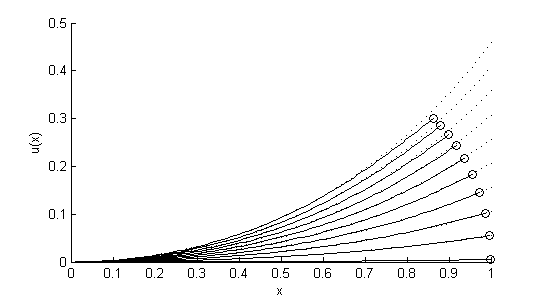
\includegraphics[width=0.60\textwidth]{./figures/lengthCorrectionErrorGraph2.png}
\end{center}
\caption[Původní ohybová funkce]%
{Původní ohybová funkce $u(x)$ pro různé výchylky (tečkovaně) a ohybová funkce po provedení korekce (plná čára). Kolečka vyznačují koncové body korigované křivky.
\label{fig:bendCorrectionGraph}
}
\end{figure}


Jak je patrné z obrázku ~\ref{fig:bendCorrectionGraph}, chyba způsobená popsanou metodou je relativně malá a nemění charakter původní ohybové křivky.

Výše popsaným způsobem získáme však ohybovou funkci pracující ve 2D. Větev je ale třeba deformovat ve 3D. Za tímto účelem jsou aplikovány dvě výše popsané deformace v navzájem kolmých osách ($r$,$s$). 

\begin{figure}[!hbt]
\begin{center}
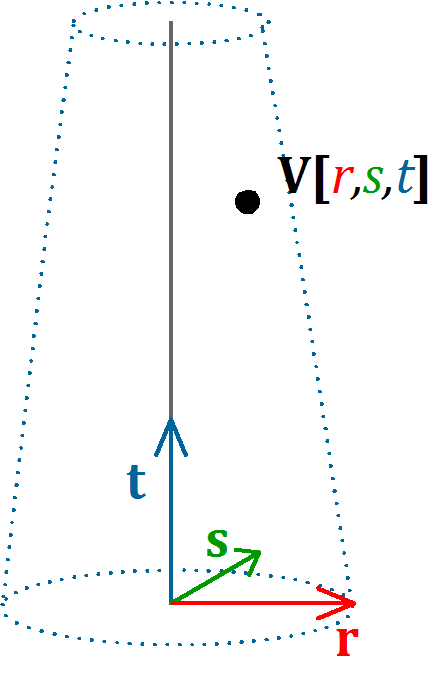
\includegraphics[width=0.2\textwidth]{./figures/branchCoords.png}
\end{center}
\caption[Souřadný systém větve]%
{Souřadný systém větve tvořený orthonormálními bázovými vektory $\vec{r}$, $\vec{s}$ a $\vec{t}$.
\label{fig:branchCoords}
}
\end{figure}

Jak vyplývá z Euler-Bernoulliho rovnice, síla ohýbající prut má lineární účinnek na ohybovou funkci – stačí tedy funkci $u(x)$ vynásobit silou $\vec{F}$, ohybová funkce závislá na síle působící na větev může být vyjádřena jako:
 \begin{equation}
\label{forceEq}
f(x) = |\vec{F}| \cdot u(x)
\end{equation}

Pokud připustíme, že síla určující výchylku je určitým řídícím signálem $A$, pak bude celková deformace řízena vztahem (indexy udávají, k jaké ose se daná funkce vztahuje):
\begin{equation}
\begin{array}{cc}
u_{r,s}(x) = A_{r,s}u(x) & {u}'_{r,s}(x) = A_{r,s}\frac{{u}'(x)}{L}
\end{array}
\end{equation}


Konečný tvar ohybové funkce pracující ve 3D je tudíž:
\begin{equation}
P = P_0 + \begin{pmatrix}
-d_r(x)/ s_r(x)-d_s(x)/s_s(x) \\ u_r(x)/s_r(x) \\ u_s(x)/s_s(x)
\end{pmatrix}
\end{equation}

Pro korektní zobrazování celé hierarchie větví je potřeba ještě správně transformovat normálu a tangentu v daném bodě $P$. Aby bylo možné korektně vyjádřit potřebné vektory, je nutné znát Jakobián $J_t$ popsané transformace. Bohužel právě jeho výpočet nelze efektivně provádět v real-time. Místo toho využijeme mnohem jednodušší Jakobián $J_u$ původní ohybové funkce (bez délkové korekce) a vyhodnotíme ho pro délkově korigovaný bod $P$.

\begin{equation}
J_{u} = \begin{pmatrix}
1 & 0 &0 \\
{u}'_r(x-d_r(x)/s_r(x)) & 1 & 0\\
{u}'_s(x-d_s(x)/s_s(x)) & 0 & 1\\
\end{pmatrix}
\end{equation}

Tangentu tedy vypočteme jako $\vec{t} = norm(J_{u}\vec{t}_{0})$, normálu pak jako $\vec{n} = norm(J_{u}^{-T}\vec{n}_{0})$

%%%%%%%%%%%%%%%%%%%%%%%%%%%%%%%%%%%%%%%%%%%%%%%%%%%%%%%%%%%%%%%%%
\subsection{Hierarchická deformace}

Předchozí kapitola popisuje, jak lze dosáhnout vcelku realistického ohybu osamocené větve. Je však třeba korektně propagovat deformaci do všech větví napojených. Pro rychlý a efektivní výpočet polohy každého vrcholu je nutné složit transformace vyplývající z topologie stromu (napojení větví a jejich ohyb). Pro každý vrchol je nutné mít přístupná data o relevantní části topologie, která ho ovlivňuje. K tomu stačí vědět, kde se větve oddělují ve smyslu parametru $x$ ohybové funkce (normovaná podélná vzdálenost na větvi). Každému vrcholu zavedeme tedy vektor hodnot $x$, kde $i$-tá složka vektoru odpovídá $i$-té hodnotě $x$ na cestě z kořene.
 
\begin{figure}[!hbt]
\begin{center}
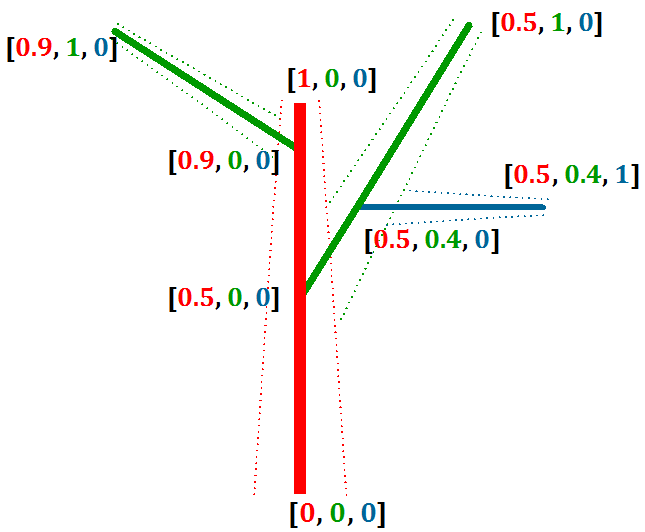
\includegraphics[width=0.5\textwidth]{./figures/branchHierarchy.png}
\end{center}
\caption[Vyjádření hierarchie]%
{ Vyjádření hierarchie pomocí vektoru s hodnotami $x$.
\label{fig:hierarchyCoords}
}
\end{figure}

Dále musí mít vrchol přiřazeny souřadnice $r$, $s$, $t$ v souřadné soustavě větve.
\begin{figure}[!hbt]
\begin{center}
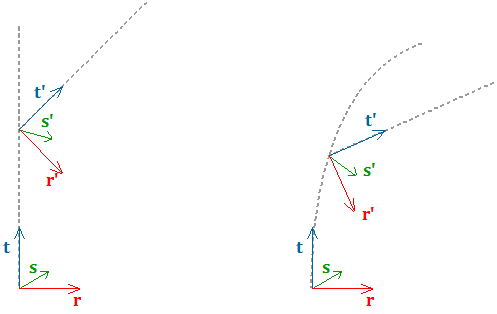
\includegraphics[width=0.5\textwidth]{./figures/coordTransf.png}
\end{center}
\caption{ Souřadný systém větve a jeho transformace při ohybu nadřazené větve
\label{fig:transfCoordSys}
}
\end{figure}	 
Aby se při ohýbání větev nezplošťovala, je nutné provádět transformaci souřadného systému větve pro každý vrchol. Zde je možnost tuto korekci neprovádět a zrychlit tak výpočet na úkor kvality výsledného ohybu.

	 
\begin{figure}[!hbt]
\begin{center}
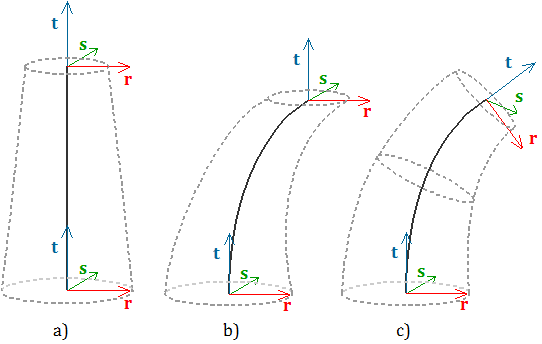
\includegraphics[width=0.5\textwidth]{./figures/branchBend.png}
\end{center}
\caption[Transformace souřadných systémů při ohybu]%
{Transformace souřadných systémů při ohybu.
(a) výchozí poloha, (b) ohyb bez transformace souřadného systému, (c) ohyb se správnou transformací
\label{fig:bendCoordSys}
}
\end{figure}

Jak je patrné z obrázku ~\ref{fig:bendCoordSys}, při malých deformacích je chyba v podstatě zanedbatelná. Při výpočtu polohy bodu $\vec{p_i}$ na středovém paprsku větve je vhodné použít následujících iterativních vztahů:

\begin{align} 
\vec{p}_{i} &= \vec{p}_{0} - \frac{\vec{t}d_{r}(x)-\vec{r}u_{r}(x)}{s_{r}(x)}-\frac{\vec{t}d_{s}(x)-\vec{s}u_{s}(x)}{s_{s}(x)}\nonumber\\
x_{i,r,s} &= x - \frac{d_{r,s}(x)}{s_{r,s}(x)}\nonumber\\
\vec{t}_{i} &=  \vec{t}_{0} + (u'_{r}(x_{i,r})\vec{r} + u'_{s}(x_{i,s})\vec{s})(\vec{t}\cdot\vec{t}_{0})\\
\vec{n}_{i} &=  \vec{n}_{0} + (u'_{r}(x_{i,r})(\vec{r} \cdot \vec{n}_{0}) + u'_{s}(x_{i,s})(\vec{s} \cdot \vec{n}_{0})\vec{t}
\end{align}

Pokud výpočet transformace polohy bodu bude probíhat od kořene hierarchie, dokud v ní není dosaženo úrovně, na které se daný vrchol nachází, pak budou postupně aplikovány všechny relevantní deformace. Na počátku je $\vec{p_0}$ původní poloha bodu v souřadném systému objektu (obdobně i tečna $\vec{t_0}$  a normála $\vec{n_0}$). V každé další iteraci (postupu o úroveň výš v hierarchii) je třeba počáteční vektory $\vec{p_0}$, $\vec{t_0}$ a $\vec{n_0}$ nastavit na výsledek z předchozí iterace. Hodnota $x_{D,r}$ a $x_{D,s}$ představuje hodnotu parametru $x$ po provedení korekce délky.  Transformace souřadného systému v rámci jedné větve vyžaduje přepočet nového bázového vektoru $\vec{t}$ podle vzorce pro výpočet tečny a nových bázových vektorů $\vec{r}$ a $\vec{s}$ podle vzorce pro výpočet normály. 

Následující tabulka shrnuje, jaká data jsou potřeba pro výpočet deformace:

\begin{table}[here]
\centering
\begin{tabular}{| l | l | }
  \hline                       
  pro vrchol & pro celou větev  \\
\hline   
  skutečná poloha & koeficienty $c_2$,  $c_4$ , délka  $L$  \\
  poloha vzhledem k větvi & definice souřadného systému větve \\
hodnota x na větvi & řídící signály ohybu \\
odkaz na větevi & odkaz na nadřazenou větev \\
  \hline  
\end{tabular}
\caption{Data potřebná k výpočtu hierarchické deformace větve}
\end{table}


%%%%%%%%%%%%%%%%%%%%%%%%%%%%%%%%%%%%%%%%%%%%%%%%%%%%%%%%%%%%%%%%
\subsection{Deformace listů}
Listy jsou součástí hierarchie stromu a musí proto respektovat i příslušný řetěz deformací této hierarchie. Kromě toho ovšem přidávají i vlastní deformaci, která je svou podstatou odlišná od deformace větví. Uplatňuje se tu jak podélná deformace, tak krut, který nastavuje plochu listu do rovnovážné polohy vzhledem k mechanickým vlastnostem a působícímu větru. 
\begin{figure}[here]
\begin{center}
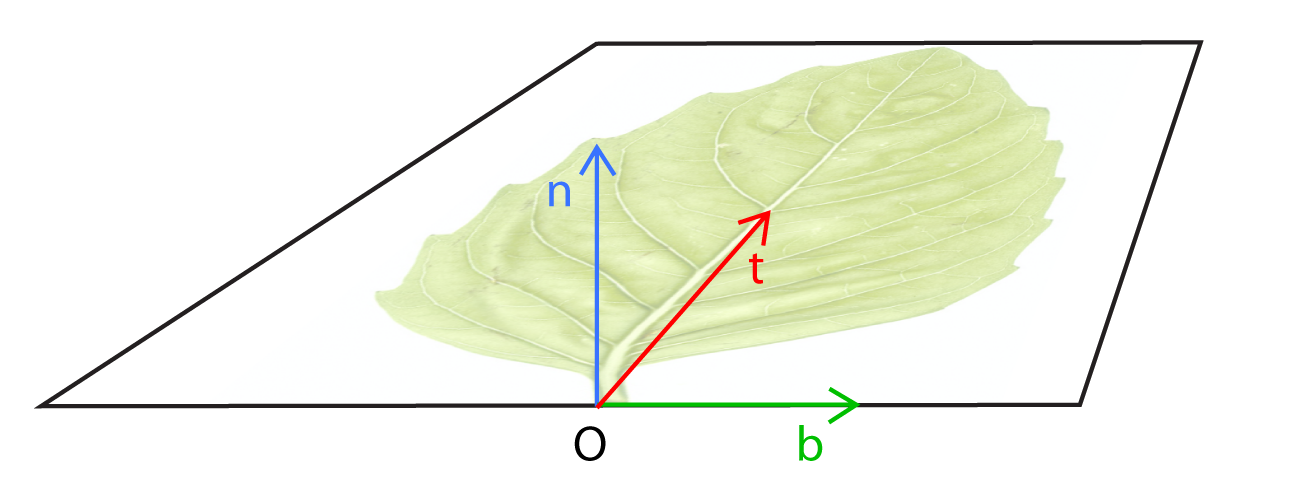
\includegraphics[width=0.45\textwidth]{./figures/leafCoordSystem2.png}
\end{center}
\caption[Souřadný systém listu]%
{ Souřadný systém listu.
\label{fig:bendLeaf}
}

\end{figure}
Jelikož považujeme listy za velice lehké a v rámci své plochy za nedeformovatelné, je tedy deformace listu aproximována jako orientace plochy listu vůči větvi, ze které vyrůstá. Jde tedy o relativně primitivní transformaci souřadného systému listu, který vytvoříme způsobem naznačeným na obrázku ~\ref{fig:bendLeaf}.


Deformace listu pak může probíhat takto:
\begin{align*} 
\vec{t}_t &= \vec{t}_0 + \vec{n}_0*A_x\\
\vec{n}_t &= \vec{t}_t \times \vec{b}_0\\
\vec{n}_r &= \vec{n}_t + \vec{b}_0*A_y\\
\vec{b}_r &= \vec{t}_t \times \vec{n}_r\\
\vec{t}_r &= \vec{t}_t
\end{align*}
\newline
\begin{equation}
P_d = O_{xyz} + P_x*\vec{b}_r + P_y*\vec{t}_r
\end{equation}
Bod $O$ je místo, kde se list napojuje na větev souřadnice $P_x$ a $P_y$ jsou dány relativně, vůči tomuto bodu v soustavě $\vec{n}\vec{b}\vec{t}$.


%%%%%%%%%%%%%%%%%%%%%%%%%%%%%%%%%%%%%%%%%%%%%%%%%%%%%%%%%%%%%%%%%%%
\subsection{Řízení animace}

Animace by měla uživateli navodit dojem, že se strom hýbe působením větru. Uvažujme, že celý pohyb je způsoben hledáním rovnovážné polohy, která závisí na mechanických vlastnostech stromu a vnějších sil (gravitace a vítr). Tím, že vnější síla v podobě působení větru je značně proměnlivá, dochází k neustálému neuspořádanému kývání kolem tušené rovnovážné polohy. Pro účely této práce dále uvažujme, že má vítr určitou složku směrového proudění  a složku turbulentního proudění. Zmíněné nahodilé kývání zřejmě způsobuje turbulentní složka, zatímco složka směrového proudění má spíše za následek celkovou změnu rovnovážné polohy (pozorovatel vnímá, že se celý strom ohýbá). 

Pozorujeme-li reálný strom, pak pro určité rozmezí malé síly větru nelze určit, kterým směrem vítr vane. V takovém případě tedy výrazně převládá vliv turbulentní složky. Lze však sledovat, že čím je daná větev větší, tím je frekvence těchto výkyvů nižší a amplituda naopak vyšší. Velikost větve odpovídá vcelku dobře její úrovni v hierarchii větví. 

Naproti tomu silnější vítr způsobí celkové ohnutí stromu do směru, kam vane. Převládá složka směrového proudění. Frekvence výkyvů jednotlivých větví se zvyšuje. Do určité meze roste i amplituda. Po jejím překročení amplituda klesá. V případě extrémní síly větru je již nahodilý pohyb větví vlivem působících sil minimální.

Popis deformací z kapitoly ~\nameref{sec-branchDeformation}  umožňuje jednoduše zohlednit obě zmiňované působící složky.
Vyjdeme-li ze vztahu \eqref{forceEq} a rozvineme sílu $\vec{F}$ do tvaru:
\begin{equation}
\label{windEq}
F_{d} = \left | \vec{W}_{turb} \right | + \vec{d}\cdot \vec{W}_{lin}
\end{equation}
bude možné promítnout sílu směrové složky větru $\vec{W}_{lin}$ a turbulentní složky $\vec{W}_{turb}$ do směru $\vec{d}$ resp. do směrů $\vec{r}$, $\vec{s}$. Aby bylo možné dosáhnout kýženého efektu způsobeného turbulentní složkou, je třeba v čase měnit příslušným způsobem sílu $\vec{W}_{turb}$. Obě složky lze chápat jako řídící signály animace (směrová složka může zůstávat konstantní). Jsou-li tyto signály měněny plynule, je plynulá i výsledná animace.

Jednotlivé větve je však třeba řídit vzájemně nezávislými signály. Proto je nutné generovat pro každou větev dvousložkový šum, který bude ideálně aperiodický a pro větev unikátní. S přihlédnutím k možnostem grafického hardwaru se jako velmi výhodná jeví strategie využívající jedinou šumovou texturu pro generování celé třídy řídících šumových funkcí. Vyhodnocením vzorku dat na určité pozici získáváme vlastně funkční hodnotu. Bude-li se pozice v textuře plynutím času posouvat po přímce definované směrovým vektorem $\vec{mv}$ (popřípadě i počátečním bodem $o$), získáme postupně funkční hodnoty průběhu požadované šumové funkce. Vzorek dat pak může obsahovat více kanálů (např. RGB, jak je u obrázků běžné) a získáme takto i více různých šumových funkcí současně, jak je patrné na obrázku \ref{fig:noiseFunctions} .
 \begin{figure}[here]
\begin{center}
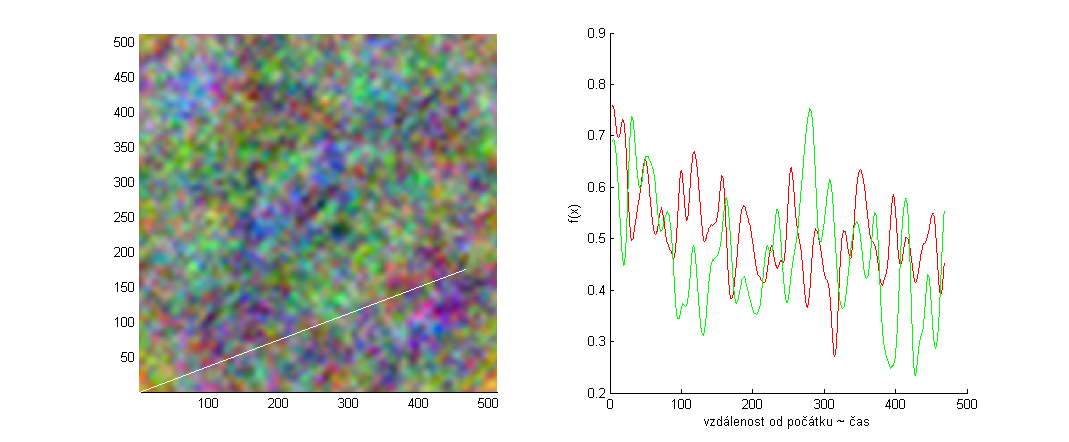
\includegraphics[width=0.85\textwidth]{./figures/noiseCut1.png}
\end{center}
\caption[Dvě generované šumové funkce]%
{ Dvě generované šumové funkce pro červený a zelený kanál (vlevo) získané odečítáním hodnot na bílé úsečce v šumové textuře (vpravo) \label{fig:noiseFunctions}
}

\end{figure}

\pagebreak
Pro pozorovatele jsou jednotlivé řídící funkce větví nezávislé – turbulentní složka je pro pozorovatele natolik chaotická, že nemůže lehce určit vzájemné vazby. Naproti tomu pro listy, které svým chováním vlastně přímo vzorkují turbulentní proudění, je dobré dodržet určité prostorové vazby. Pozorovatel totiž dokáže rozeznat poryv větru docela dobře podle pohybu listů. Listy v blízkém okolí musí na poryv reagovat podobně. Z toho důvodu zavedeme zjednodušený model turbulentního pole (viz obrázek ~\ref{fig:TurbulentFieldModel}). 
\begin{figure}[!hbt]
\begin{center}
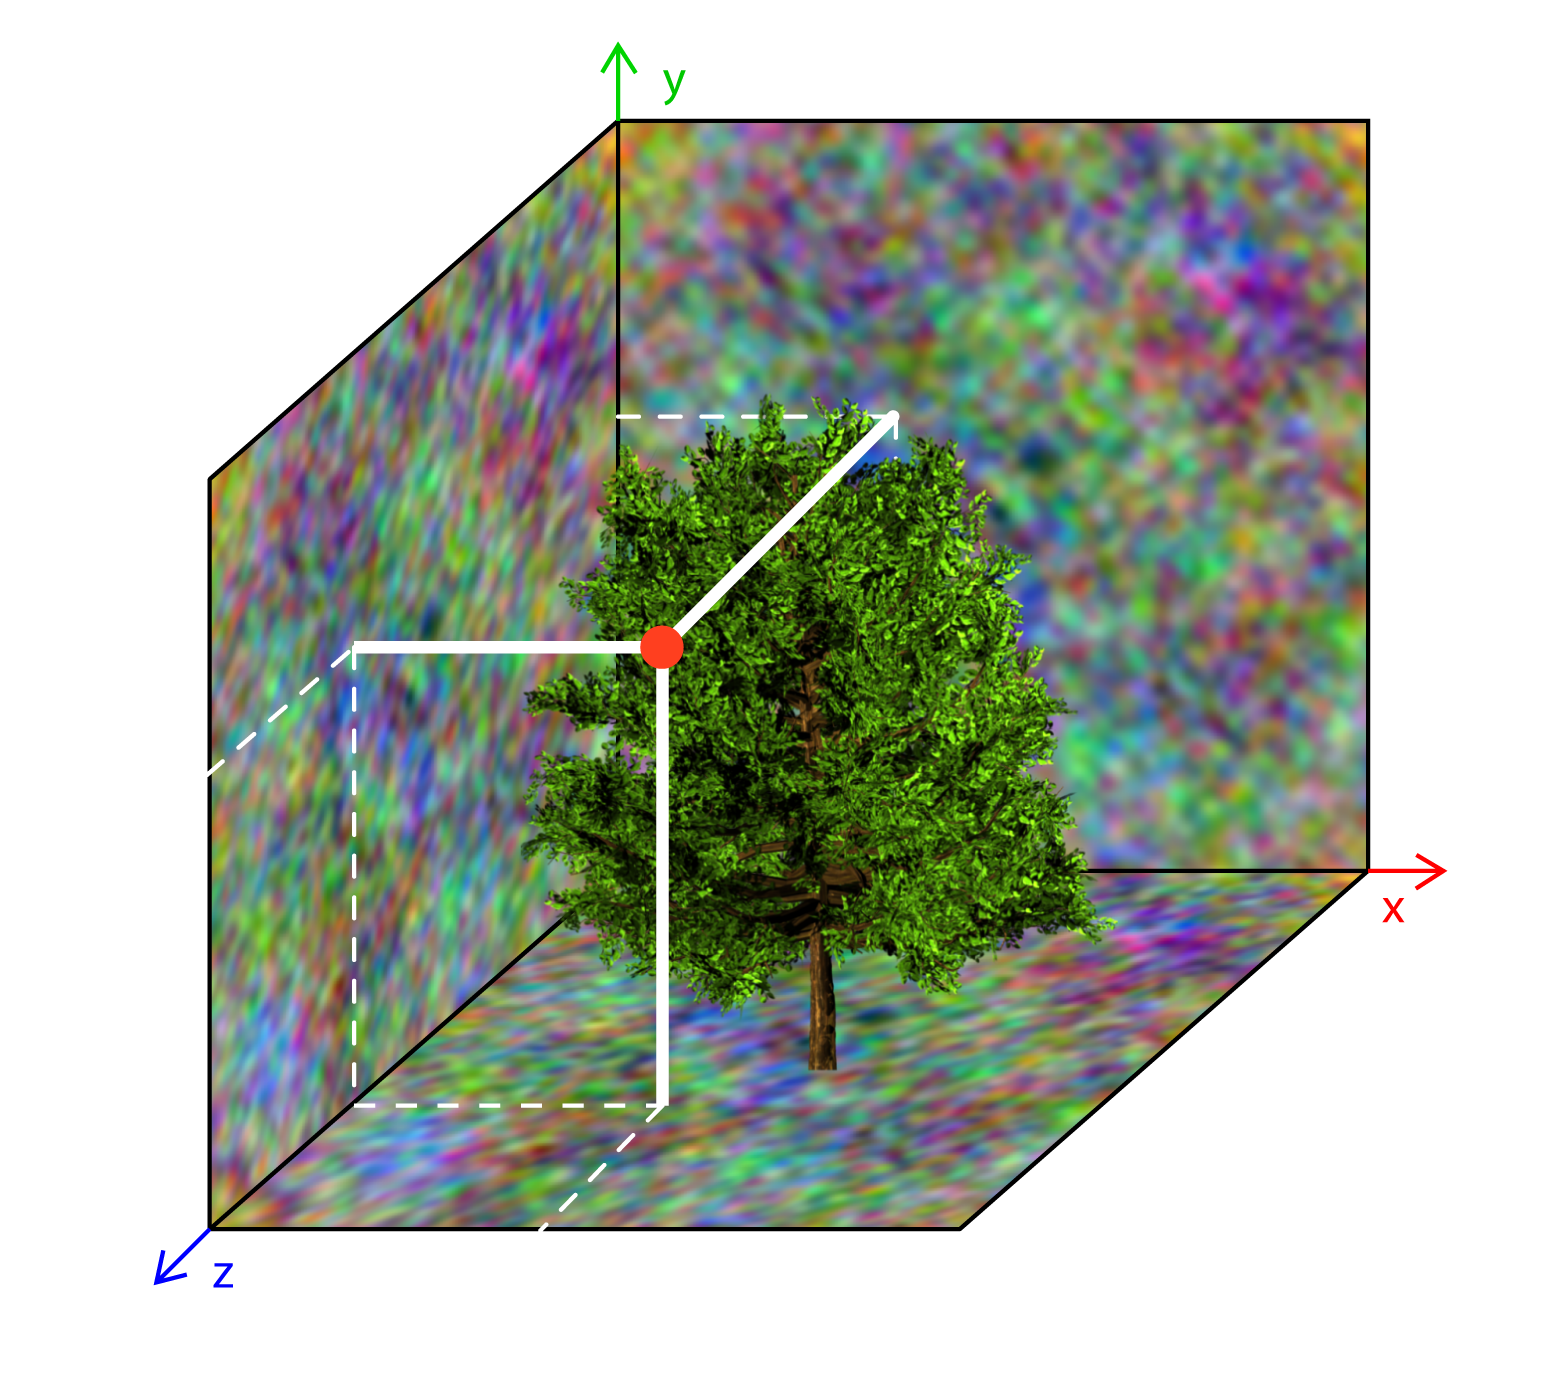
\includegraphics[width=0.5\textwidth]{./figures/turbulentField.png}
\caption[Model 3D turbulentního pole]%
{Model 3D turbulentního pole pro animaci listů\label{fig:TurbulentFieldModel}}
\end{center}

\end{figure}

 K tomu lze využít jedinou šumovou texturu. Pozici dotazu do turbulentního pole posuneme o vektor $-\vec{W} \cdot t$, kde $t$ je čas. Získáme tak 3 hodnoty $A_{xy,xz,yz}$, ze kterých vypočteme vážený součet. 
\begin{equation}
 A^{l} = A^p_{xy}(1-\frac{\left | W_z\right |}{\left | \vec{W}\right |})
+ A^p_{yz}(1-\frac{\left | W_x\right |}{\left | \vec{W}\right |}) +
A^p_{xz}(1-\frac{\left | W_y\right |}{\left | \vec{W}\right |})
\end{equation}
Výsledkem je hodnota, která je největším dílem tvořena z roviny, jež nejlépe odpovídá směru větru.


% Zobrazování listů %%%%%%%%%%%%%%%%%%%%%%%%%%%%%%%%%%%%%%%%%%%%%%%%%%%
\section{Zobrazování listů}
\label{sec-leafMethod}
Listy rostlin představují z hlediska počítačové grafiky zajímavý objekt. Jejich vizuální vlastnosti se liší mezi jednotlivými druhy rostlin. Zároveň je často velmi markantní rozdíl mezi rubovou (horní) a lícovou (spodní) stranou. Zatímco zvrchu jsou některé listy vysoce lesklé díky různým voskovým vrstvičkám, zespodu jsou často spíše matné. Některé listy mají na povrchu miniaturní chloupky, které jim dávají hedvábný vzhled. Dalšími faktory jsou pak tvar, tloušťka a barva listu. 
 \begin{figure}[here]
\begin{center}
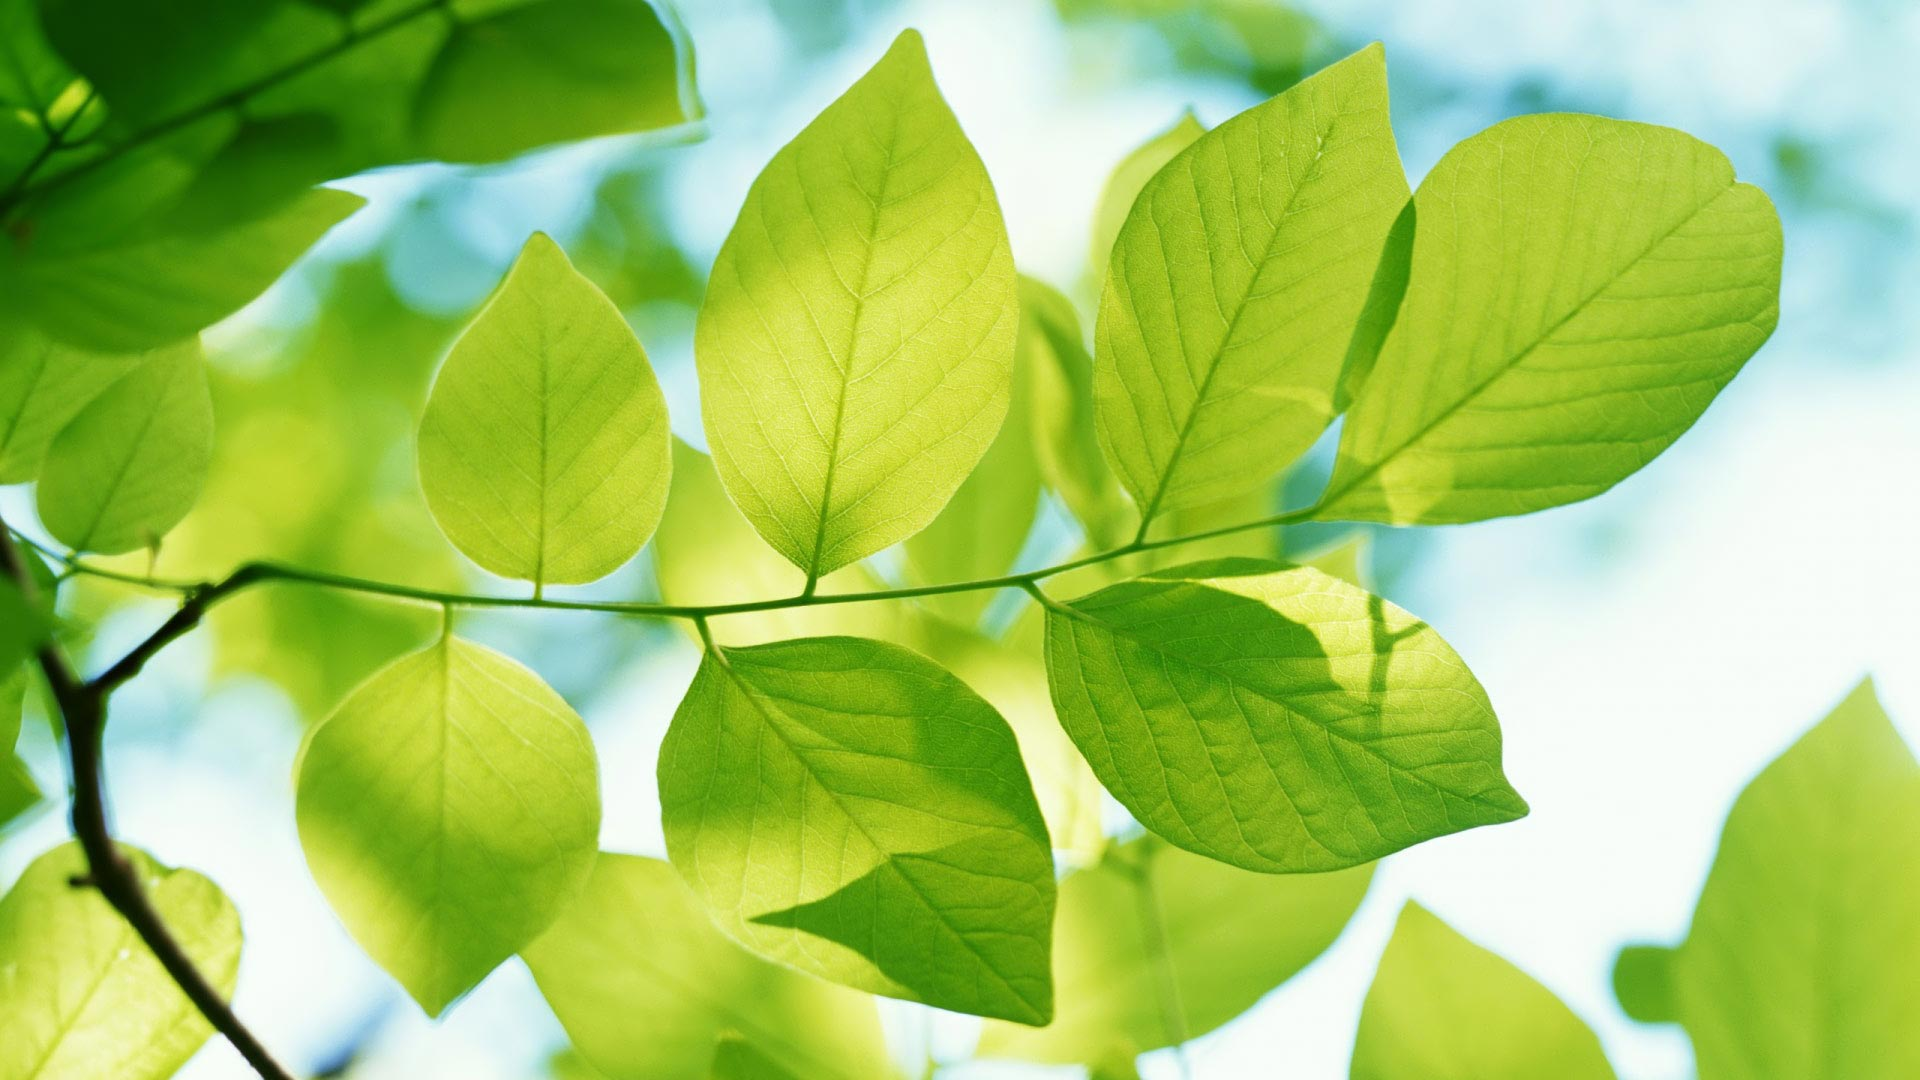
\includegraphics[width=0.5\textwidth]{./figures/translucent_leaves.jpg}
\end{center}
\caption{ Fotografie skutečných listů, kde se projevuje jejich průsvitnost, zdroj \cite{TLW} \label{fig:translucentLeaves}
}

\end{figure}

Metod a postupů, jak zobrazovat listy v real-time existuje několik. Většina přístupů se ale spokojuje s tím, že bere v potaz pouze povrchové vlastnosti listu a simuluje tak například členitost jeho povrchu či běžné odrazové vlastnosti. Metoda popsaná v \cite{Habel_2007_RTT} ovšem zahrnuje i průsvitnost listů, která hraje zásadní roli zejména na spodní straně listu (viz obr. \ref{fig:translucentLeaves}). Osvětlení listu lze zformulovat do následujícího vztahu
\begin{equation}
L = L_D + L_I + L_E,
\end{equation}
kde výsledné osvětlení $L$ z jednoho světelného zdroje se skládá z příspěvku přímého ($L_D$) a nepřímého ($L_I$) osvětlení a složky $L_E$, kterou list emituje. 
V následujícím textu bude rozebrán pouze příspěvek přímého osvětlení. Zbylé budou aproximovány ambientní složkou. Přímé osvětlení lze pak schematicky rozepsat jako:
\begin{equation}
\label{eq:directLight}
L_D = L_{diffuse} + L_{specular}+ L_{ambient} + L_{translucent},
\end{equation}
kde první tři členy představují příspěvek odraženého světla, zatímco poslední člen $ L_{translucent}$ se vztahuje k průsvitnosti listu.

K vyjádření difuzní a spekulární složky využijeme popisu z obrázku \ref{fig:lightModel}.
 \begin{figure}[here]
\begin{center}
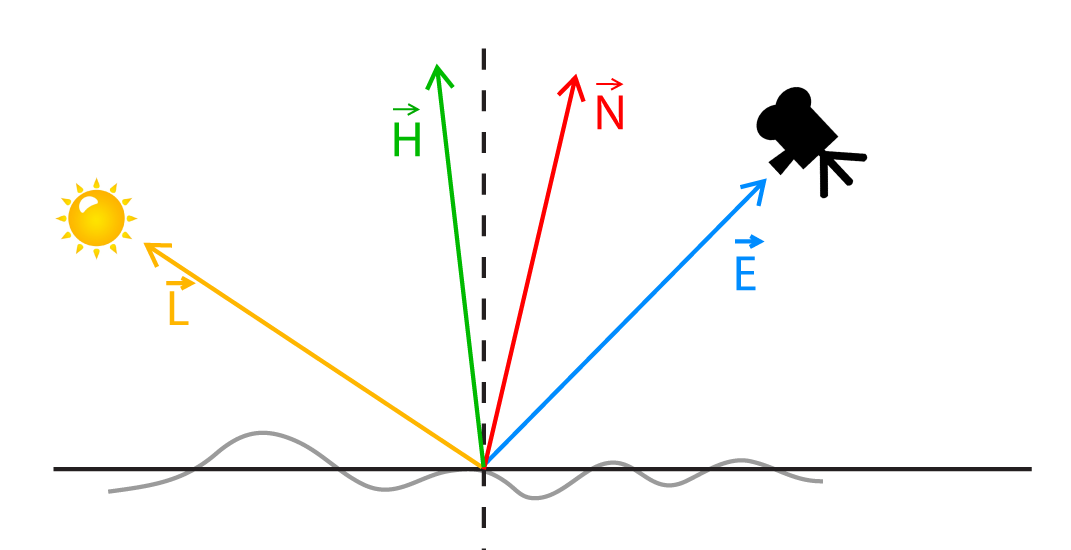
\includegraphics[width=0.5\textwidth]{./figures/lightModel.png}
\end{center}
\caption[Situace na povrchu listu]
{Situace na povrchu listu.  Vektor $\vec{N}$ definuje normálu v bodě dopadu paprsku. $\vec{E}$ udává směr k pozorovateli a $\vec{L}$ ke světlu. Vektor $\vec{H}$ je definován na ose úhlu mezi $\vec{L}$ a $\vec{E}$. Šedivá křivka představuje povrch.\label{fig:lightModel}
}
\end{figure}
Difuzní složku lze určit jako příspěvek světla vážený úhlem mezi přicházejícím paprskem světla $\vec{L}$ a normálou povrchu $\vec{N}$ v místě jeho dopadu:
\begin{equation}
L_{diffuse} = \vec{N} \cdot \vec{L}
\end{equation}
Výpočet spekulární složky je oproti tomu složitější. Nevyužívá Phongova osvětlovacího modelu, ale nahrazuje ho odvozeninou osvětlovacího modelu Cook-Torrance popsaného v \cite{Cook:1981:RMC:965161.806819} a \cite{Bousquet2005201}. Tento model pracuje s BRDF jež operuje nad proměnými $\vec{N}$, $\vec{L}$, $\vec{E}$, $\vec{H}$ (význam viz obr. \ref{fig:lightModel}), $\sigma$ udávajícím drsnost povrchu a indexem lomu $n$ světla na povrchu listu.

\begin{equation}
\label{eq:brdf}
BRDF_{spec}(\vec{N}, \vec{L}, \vec{E}, \vec{H}, \sigma, n) = \frac{R(\sigma, \vec{N}, \vec{H}) \cdot F(n, \vec{H}, \vec{E}) \cdot G(\vec{N}, \vec{L}, \vec{E},\vec{H}) }{(\vec{N}\cdot\vec{L})(\vec{N}\cdot\vec{E})\pi}
\end{equation}
Člen $R(\sigma, \vec{N}, \vec{H})$ představuje vliv hrubosti povrchu a může být vyjádřen jako:
\begin{equation}
\label{eq:roughness}
R(\sigma, \vec{N}, \vec{H}) = \frac{1}{\sigma^2 \cdot ( \vec{N}\cdot\vec{H})^4} \cdot e^{\left ( \frac{\frac{1}{ ( \vec{N}\cdot\vec{H})^2} -1}{\sigma^2}\right )}
\end{equation}
Naproti tomu, člen $F(n, \vec{H}, \vec{E})$ popisuje lesklou složku:
\begin{align}
\label{eq:fresnel}
c &= \vec{H} \cdot \vec{E} \nonumber\\
g &= \sqrt{n^2 + c^2 - 1}\nonumber\\
F(n, \vec{H}, \vec{E}) &= \frac{1}{2} \left ( \frac{g-c}{g+c} \right)^2 \left [  1+ \left( \frac{c (g+c)-1}{c(g-c)+1}\right)\right ]
\end{align}
Konečně člen $G(\vec{N}, \vec{L}, \vec{E},\vec{H})$ popisuje geometrii v bodě dopadu paprsku:
\begin{equation}
\label{eq:geometry}
G(\vec{N}, \vec{L}, \vec{E},\vec{H}) = \min{} \left( 1, \frac{2\cdot(\vec{N}\cdot\vec{H})\cdot(\vec{N}\cdot\vec{E})}{(\vec{E}\cdot\vec{H})}, \frac{2\cdot(\vec{N}\cdot\vec{H})\cdot(\vec{N}\cdot\vec{L})}{(\vec{E}\cdot\vec{H})} \right)
\end{equation}

Složka způsobená průsvitností listu má dominantní vliv, pokud se světelný zdroj nachází za rovinou listu vzhledem k pozorovateli. K jejímu vyjádření je použit BSSRDF model. Jeho konstrukcí a určením pro různé listy se věnuje \cite{Habel_2007_RTT} a tato problematika zde nebude dále rozebírána. Zmiňovaná funkce $L_t$ závisí na pozici $\vec{x}_0$, směru k pozorovateli $\vec{E}$ a směru ke světlu $\vec{L}$ a může být napsána v diskrétní formě takto:
\begin{equation}
\label{eq:bssrdf}
L_t(\vec{x}_0, \vec{E}, \vec{L}) = \rho_t(\vec{x}_0, \vec{E}) A_p \sum\limits_{\vec{x}_i} T(r, d(\vec{x}_i))E(\vec{x}_i, \vec{L}),
\end{equation}
kde $\rho_t(\vec{x}_0, \vec{E})$ reprezentuje propustnost, $A_p$ zastupuje plochu texelu, $T(r, d(\vec{x}_i))$ je dynamické konvoluční jádro díky závislosti na tloušťce listu $d(\vec{x}_i)$ a konečně $E(\vec{x}_i, \vec{L})$ je přenosová funkce osvitu (irradiance transport function). Jde v zásadě o proces konvoluce obrazové informace a můžeme tedy odlišit konvoluční část.
\begin{align}
\label{eq:bssrdf_convol}
L_t(\vec{x}_0, \vec{E}, \vec{L}) &= \rho_t(\vec{x}_0, \vec{E}) L_t^C( \vec{x}_0, \vec{L}) \\
L_t^C( \vec{x}_0, \vec{L})  &= A_p \sum\limits_{\vec{x}_i} T(r, d(\vec{x}_i))E(\vec{x}_i, \vec{L}),
\end{align}
 Právě konvoluční část tvořená hemisférickou funkcí $L_t^C$ je v real-time příliš obtížné vypočíst, a proto se předpočítá pro každý texel. Reprezentována pak je pomocí tzv. \emph{Half Life 2 bází} (HL2b). Jde o konstrukt, který umožňuje jednoduše vyjádřit reprezentovanou funkci pro daný hemisférický směr. Bázové vektory HL2b jsou následující:
\begin{align}
\label{eq:hl2b_vectors}
\vec{H}_1 &= (-\frac{1}{\sqrt{6}}, -\frac{1}{\sqrt{2}}, \frac{1}{\sqrt{3}}) \nonumber\\
\vec{H}_2 &= (-\frac{1}{\sqrt{6}}, \frac{1}{\sqrt{2}}, \frac{1}{\sqrt{3}}) \nonumber \\
\vec{H}_3 &= (\sqrt{\frac{2}{3}}, 0, \frac{1}{\sqrt{3}})
\end{align}
Tyto vektory pak definují tři kosínové bázové funkce na polokouli (hemisféře):
\begin{equation}
\label{eq:hl2b_cosineFunctions}
\mathcal{H}_i(\vec{d}) = \sqrt{\frac{3}{2\pi}}\vec{H}_i \cdot \vec{d}
\end{equation}
Hemisférickou funkci $f(\vec{d})$ pro směr $\vec{d}$  lze tedy přepsat pomocí těchto bázových funkcí následovně:

\begin{equation}
\label{eq:hl2b_function}
f(\vec{d}) = \sum\limits_{i=1\dots3}h_i\mathcal{H}_i(\vec{d}),
\end{equation}
kde $h_i$ jsou souřadnice vzhledem k bázovým funkcím.

Výsledný vztah rekonstruující původní $L_t$ využívající HL2b pro předpočítanou konvoluční funkci pak vypadá takto:
\begin{equation}
\label{eq:hl2b_use}
L_t^R(\vec{x}_0, \vec{L}) = L_D \rho(\vec{x}_0) \sum\limits_{i=1\dots3}h_i(\vec{x}_0)\sqrt{\frac{3}{2\pi}}\vec{H}_i \cdot  \vec{L}
\end{equation}
Uvážíme-li, že $L_D \rho(\vec{x}_0)$ a $h_{1\dots3}(\vec{x}_0)$ lze uložit do textur (pro pozici $\vec{x}_0$), lze tím pádem průsvitnost vypočíst na základě pouze dvou dotazů do textur.

Posledním krokem je přizpůsobit výše popsané postupy tak, aby bylo možné dynamicky měnit barvu listů. Barva se liší jednak v rámci jednoho listu, jednak mezi listy. Sezónní změny barvy listu se často projevují různě v různých částech listu. Zatímco okrajové části mohou být už červené či žluté, středové části mohou zůstávat stále zelené. Toto chování ovšem není cílem napodobit. Důraz bude kladen na celkovou barevnost listu, která hraje roli při pohledu z větší vzdálenosti.
\begin{figure}[here]
\begin{center}
$\begin{array}{cc}
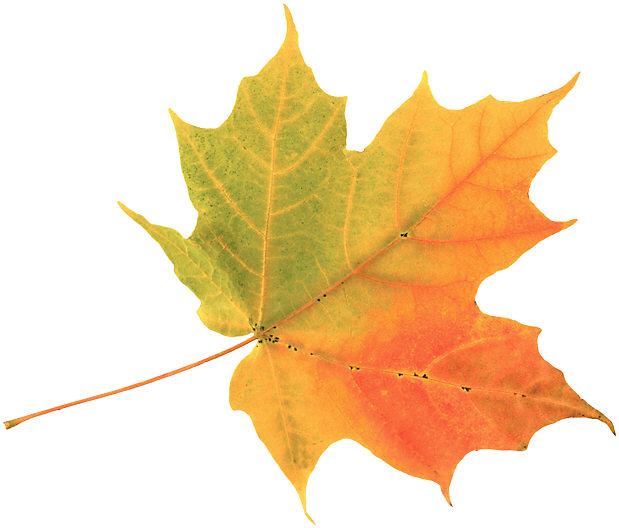
\includegraphics[width=0.4\textwidth]{./figures/fall-leaf.jpg}&
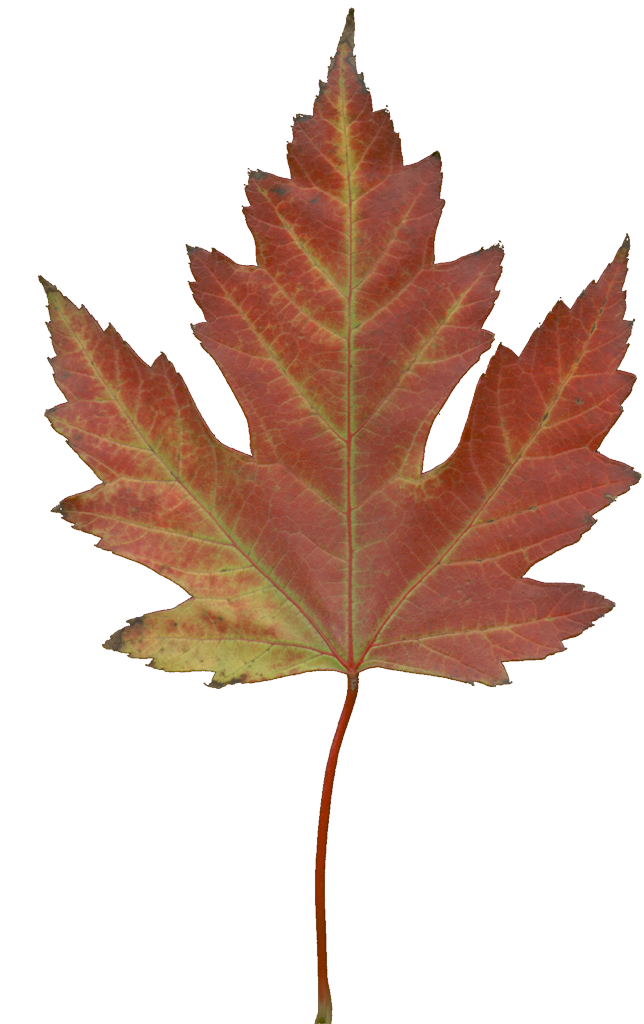
\includegraphics[width=0.3\textwidth]{./figures/fall-leaf2.png}
\\
(a)&(b)
\end{array}$
\end{center}
\caption{ Fotografie skutečných listů, barevné variace v ploče listu\label{fig:fallLeaves}
}
\end{figure}

Vyjdeme-li ze vztahu \ref{eq:directLight}, a budeme-li ho chápat pouze jako jednotlivé skalární podíly intenzit světla, můžeme vytvořit následující vztah pro zahrnutí barevnosti listu: 
\begin{equation}
\label{eq:color_solution}
L_D = L_{diffuse}  \mathcal{D} + L_{specular} \mathcal{S} + L_{ambient} \mathcal{A}   + L_{translucent} \mathcal{T} ,
\end{equation}
přičemž $\mathcal{D}$ je difuzní barva v daném bodě, $\mathcal{S}$ je barva odlesku daná barvou světelného zdroje a materiálem, $\mathcal{A}$ je barva ambientního příspěvku světla a $\mathcal{T}$ je barva vzniklá průchodem světla listem.

 Pro konkrétní bod $x$ a sezónu $s$ lze barvy vyjádřit jako:
\begin{align}
\label{eq:color_def}
\mathcal{D}(x,s) &= (c_v(x) + c_s(s))\cdot \mathcal{M}_{diffuse}\nonumber\\
\mathcal{A}(x,s) &= (c_v(x) + c_s(s))\cdot \mathcal{M}_{ambient}\nonumber\\
\mathcal{S}(x,s) &= \mathcal{M}_{specular}\nonumber\\
\mathcal{T}(x,s) &= (c_t(x) + c_s(s))\cdot \mathcal{M}_{translucent} ,
\end{align}
kde $ \mathcal{M}_{(\dots)}$ je pro daný materiál na světelný zdroj konstanta, $c_v(x)$ je prostá barva listu, která je definovaná texturou, $c_s(x)$ je barevná odchylka daná sezónními změnami barvy (dovolíme si zjednodušení: sezónní barevná odchylka je pro celý list stejná ). Člen $c_t(x)$ vyjadřuje barvu po průchodu světla listem, která je rovněž definovaná texturou. Na tomto místě je dobré přiznat, že správnější by bylo uvažovat pro různé barevné variace listu dané sezónou i různé barvy průsvitné složky. Řešní by se tím ovšem zkomplikovalo a i popsaný přístup funguje relativně dobře.
Předpokládá se, že každá ze dvou stran listu bude vyhodnocována odděleně s jinými parametry (různé textury, příp. materiály). Na obrázku \ref{fig:leafResources} jsou zdrojové textury pro jednu stranu listu.
\begin{figure}[here]
$\begin{array}{cccc}
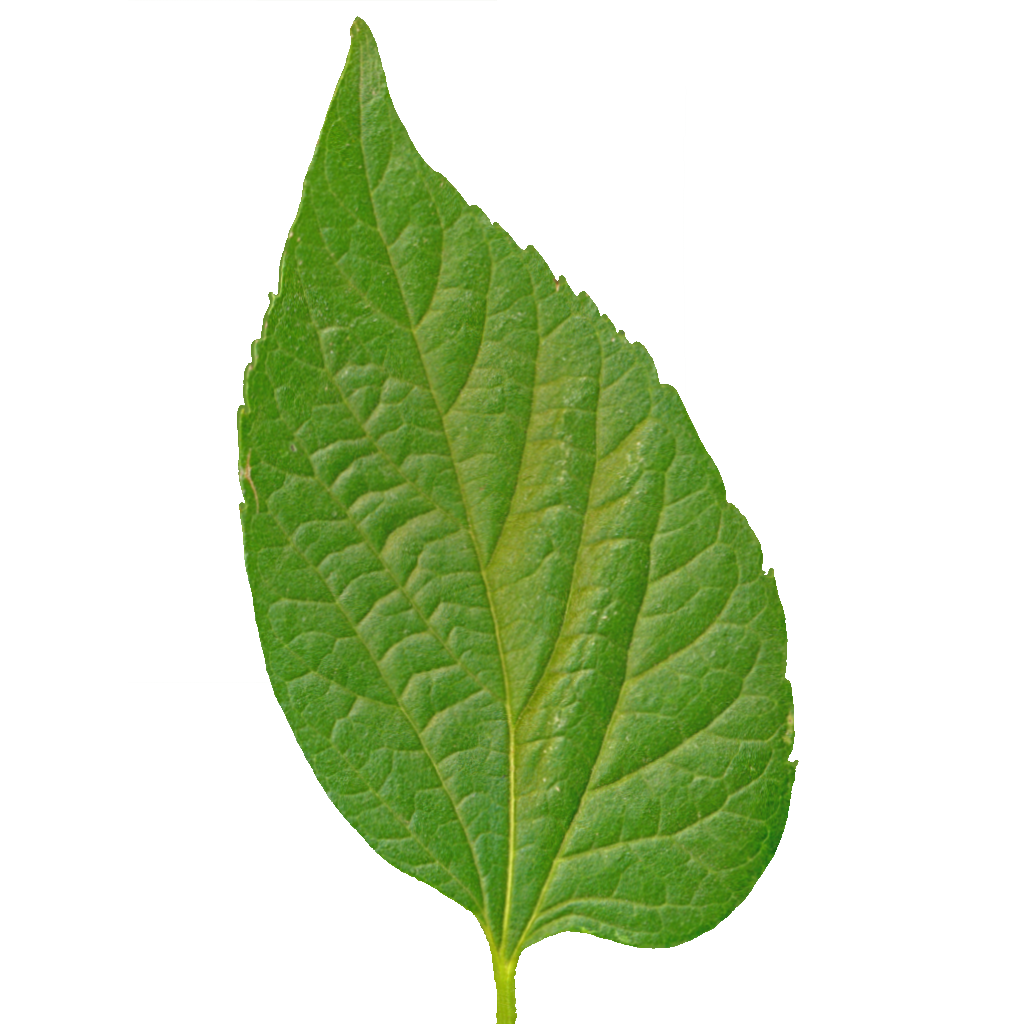
\includegraphics[width=0.2\textwidth]{./figures/leaf3_decal_front.png}&
&
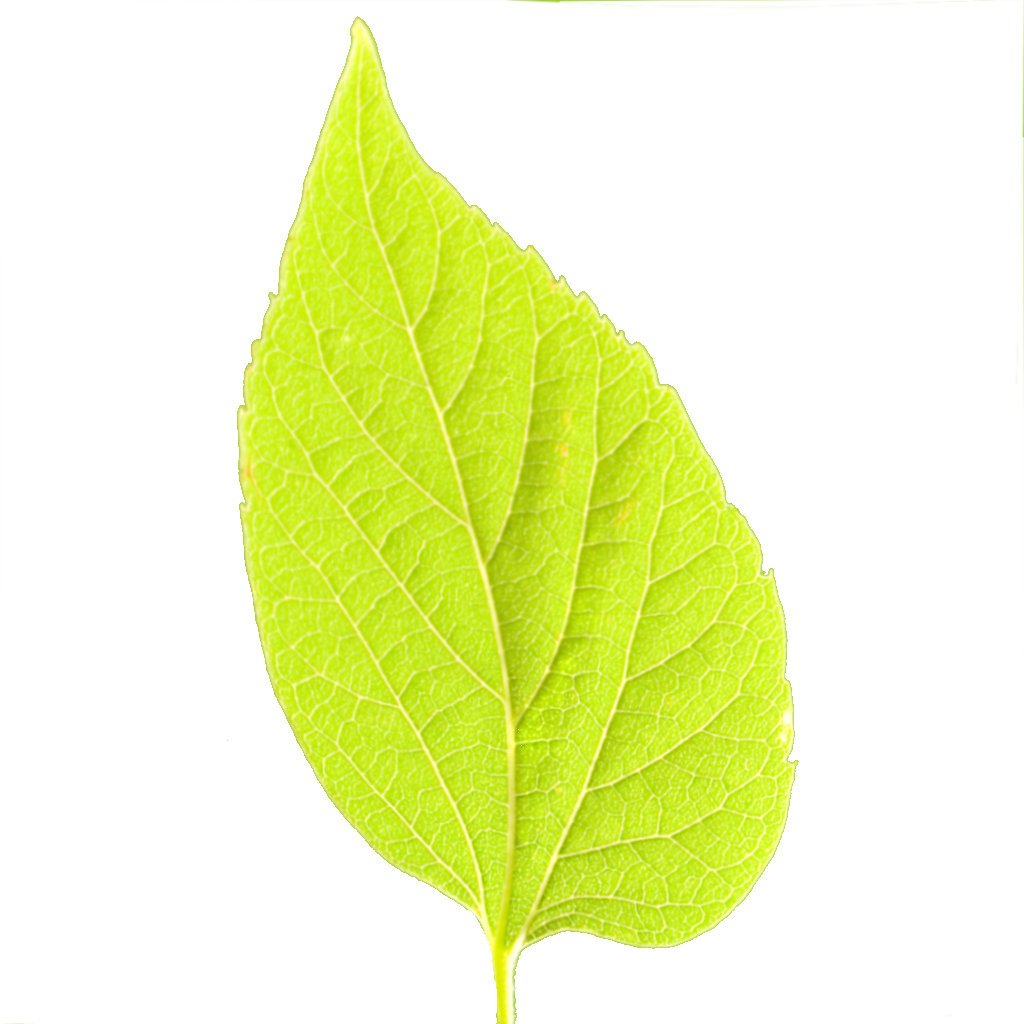
\includegraphics[width=0.2\textwidth]{./figures/leaf3_translucency_front.png}&
\\
(a)&&(b)&
\\
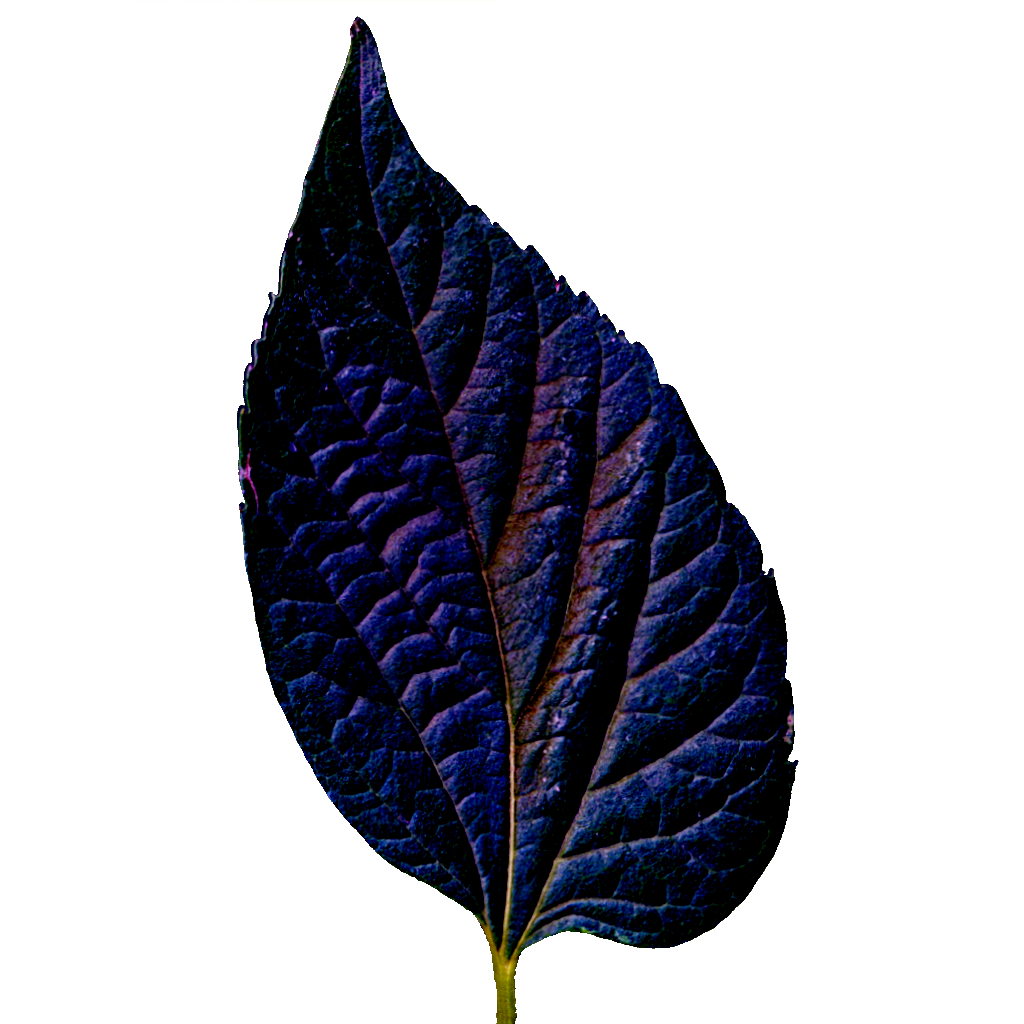
\includegraphics[width=0.2\textwidth]{./figures/leaf3_decal_front_e.png}&
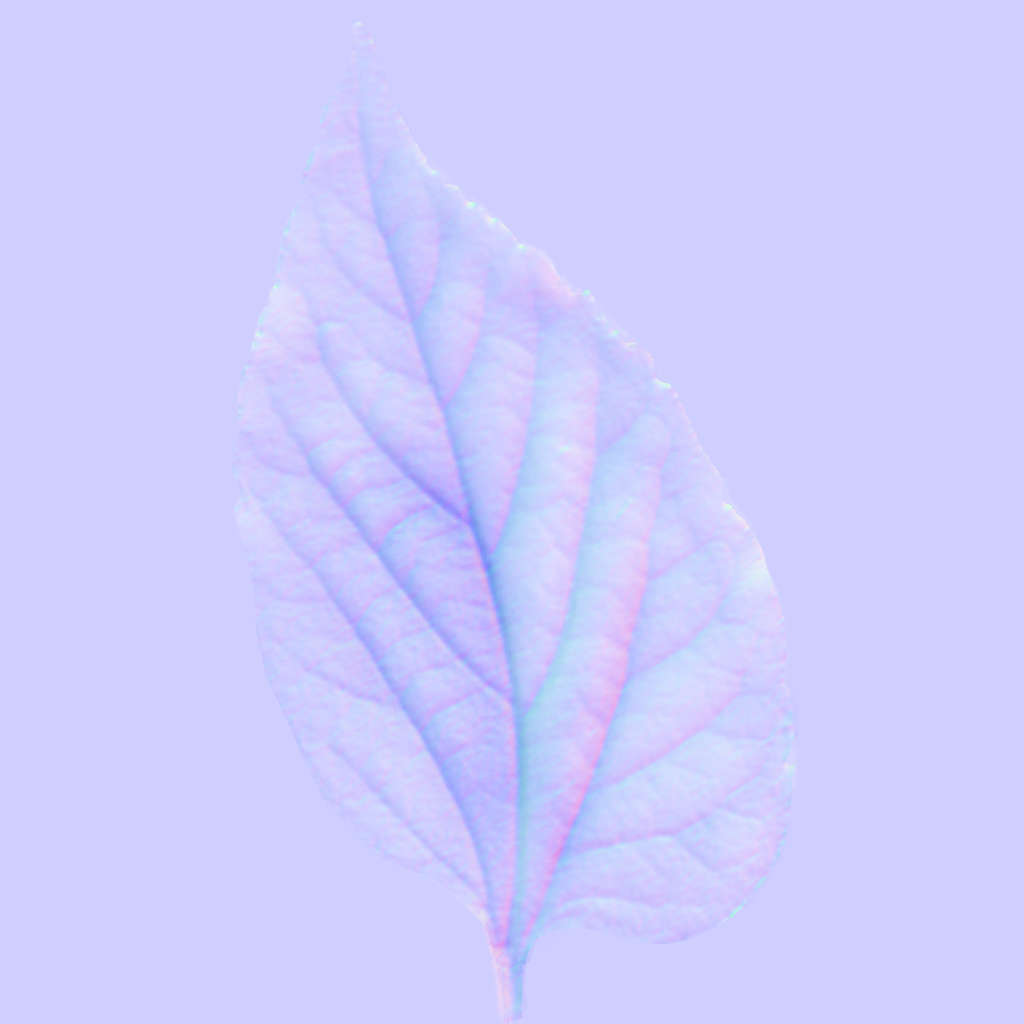
\includegraphics[width=0.2\textwidth]{./figures/leaf3_normal_front.png}&
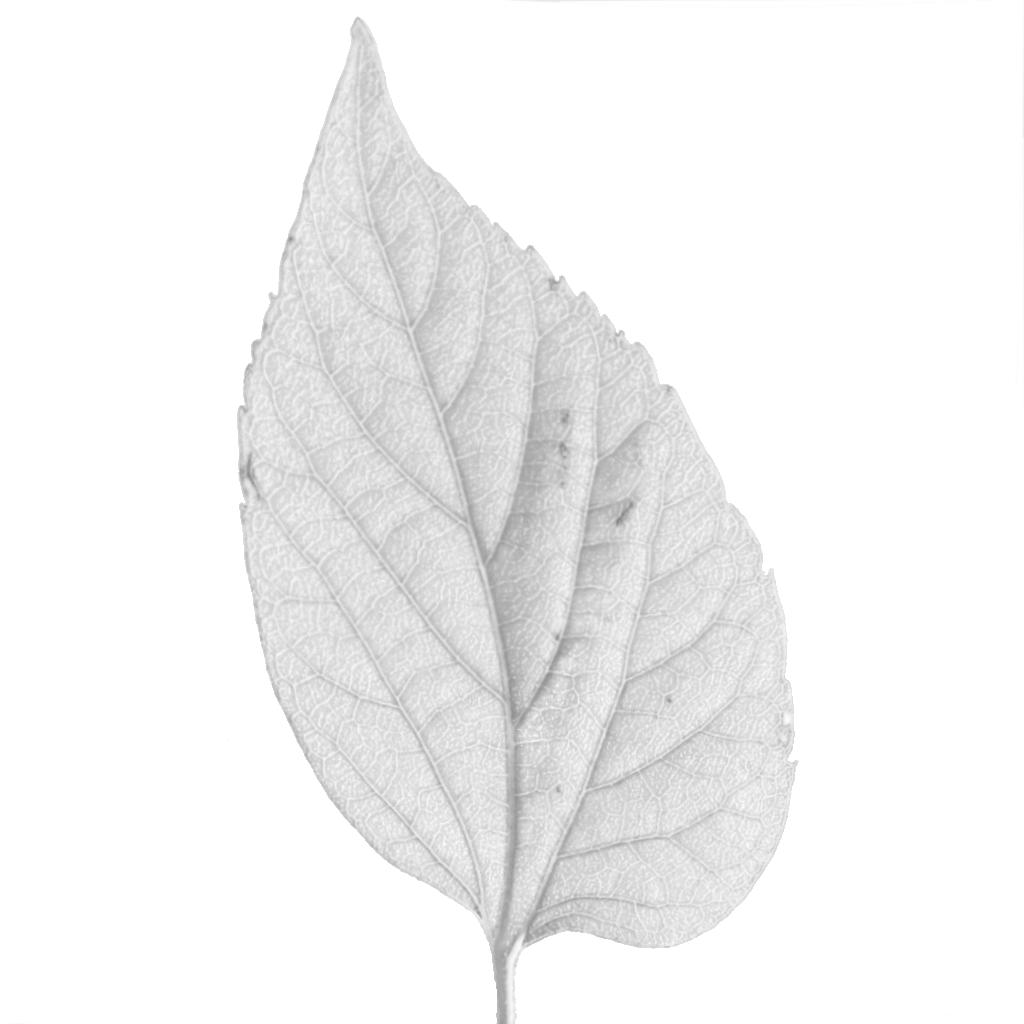
\includegraphics[width=0.2\textwidth]{./figures/leaf3_translucency_front_e.png}&
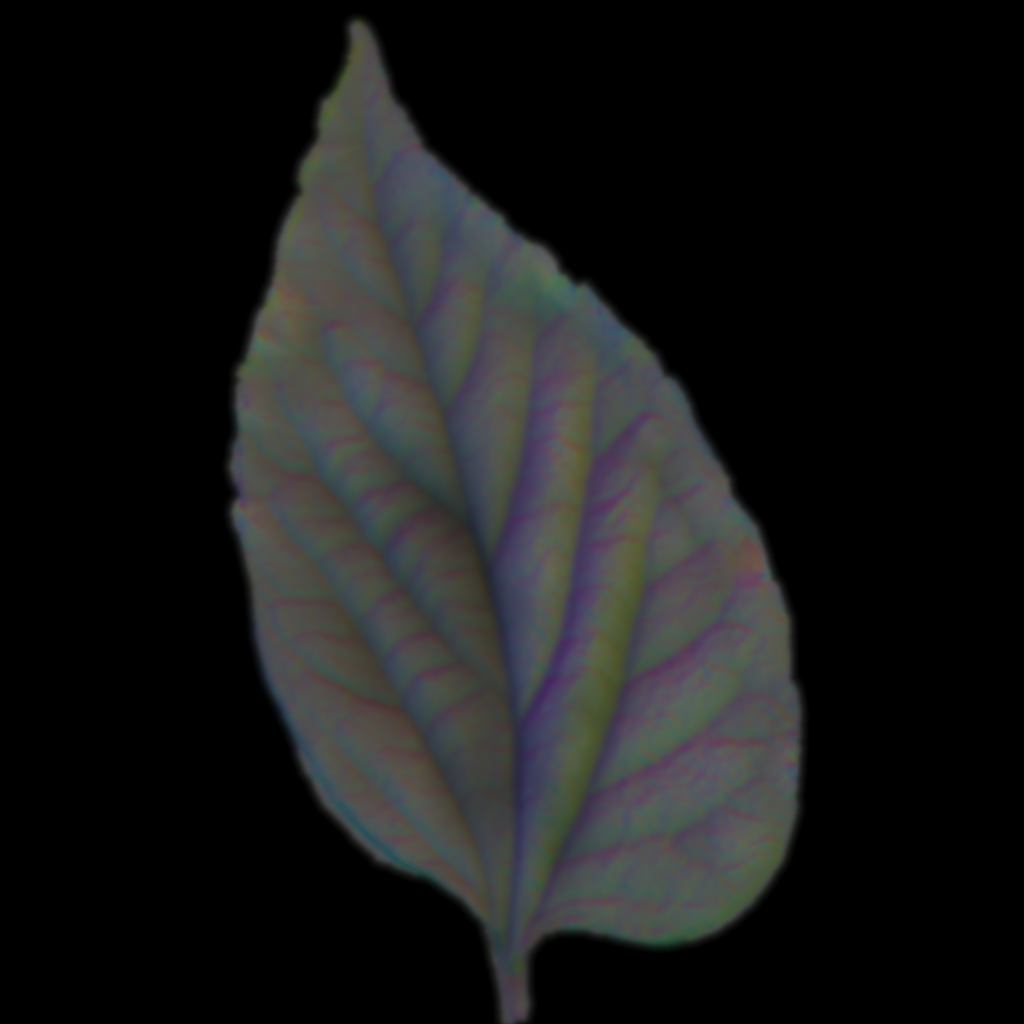
\includegraphics[width=0.2\textwidth]{./figures/leaf3_halflife2_front.png}
\\
(c)&(d)&(e)&(f)
\end{array}$
\caption[Zdrojové textury pro výpočet osvětlení listů]%
{Zdrojové textury pro výpočet osvětlení listů. (a) původní barevná mapa, (b) původní mapa průsvitnosti, (c) mapa barevných odchylek od základní barvy listu (pro názornost zvětšeny), (d) normálová mapa, (e) mapa průsvitnosti, (f) mapa koeficientů Half Life 2 bázových funkcí \label{fig:leafResources}
}
\end{figure}
Pro listy jsou ovšem k dispozici původně jiná zdrojová data. Původní barevná mapa obsahuje prosté barvy listu (např. fotografie) - jde vlastně o záznam podoby listu pro jednu sezónní barvu a tu neumožňuje přímo a jednoduše dynamicky měnit. Mapu barevných odchylek můžeme získat z původní barevné mapy odečtením základní barvy listu (později přičtena jako sezónní barva listu). Obdobné předzpracování je nutné provést s původní mapou průsvitnosti, na kterou je výhodnější nahlížet jako na mapu intenzit.  

\newpage



% LOD %%%%%%%%%%%%%%%%%%%%%%%%%%%%%%%%%%%%%%%%%%%%%%%%%%%%%%%%%
\section{Úrovně detailu}
\label{sec-LOD}
V předchozích kapitolách předpokládáme zpracování a zobrazování geometrického modelu vegetace. Pro nižší úrovně detailu (LOD) lze využít metod, které složitou geometrii typicky nahrazují zobrazením primitivní geometrie (např. čtverce), na které je aplikována textura (obrázek) navozující dojem, že se jedná o původní objekt. Zaznamenáme-li pohledy na objekt z několika směrů, lze s určitou rozumnou tolerancí ke snížení kvality zobrazit následně pomocí těchto pohledů libovolný pohled na objekt bez nutnosti zobrazení a zpracování jeho plné geometrické reprezentace. Úspora potřebného výkonu spočívá jak v malém počtu zpracovávaných vrcholů geometrie, tak v ušetření řady rasterizačních operací stejně jako v menším počtu zpracovávaných fragmentů.
\footnote{ předpokládá se, že jednotlivé listy jsou vykreslovány v náhodném pořadí a tím pádem je barva určitého pixelu několikrát přepisována}
 Výsledná kvalita zobrazeného objektu je ovlivněna počtem předgenerovaných pohledů, jejich kvalitou a také způsobem, jak zkonstruovat obraz pro pohled ze směru, pro který neexistuje předgenerovaný obraz.
Známé jsou metody billboardingu využívající pro osově souměrnou geometrii jediného pohledu, který je natáčen kolmo k pohledu virtuální kamery. \footnote{existuje několik možností natáčení obrázku např:
\begin{itemize}
\item rovnoběžně se stínítkem kamery
\item kolmo k pohledu kamery
\end{itemize}
}
Relativně běžná je metoda využívající jakýchsi trsu billboardů. Objekt je nahrazen množinou různě orientovaných geometrických primitiv, jak je patrné z obrázku 
\begin{figure}[!hbt]
\begin{center}
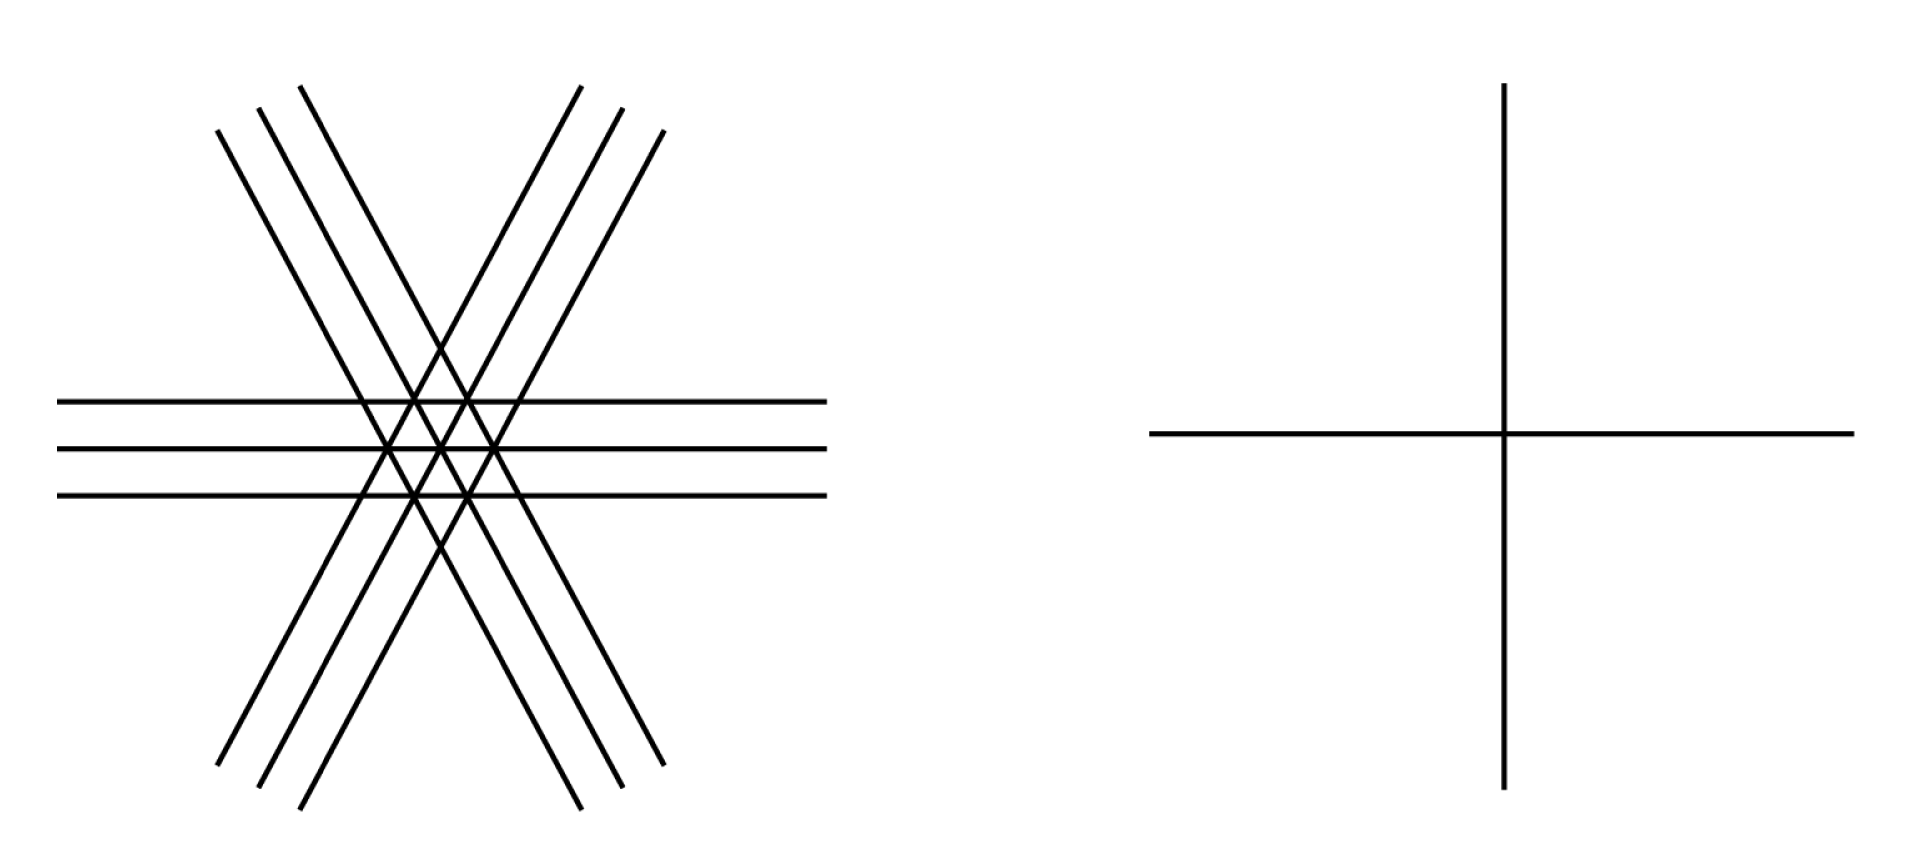
\includegraphics[width=0.75\textwidth]{./figures/slicesTop.png}
\caption{ Konstrukce jednoduchého trsu billboardů: (pohled zvrchu) vyšší LOD tvořený třemi skupinami billboardů po 3 řezech (vlevo), nižší LOD tvořený pouze dvěma kolmými billboardy (vpravo) }
\end{center}
\label{fig:sliceBilboard}
\end{figure}

Na rozdíl od metod skutečného billboardingu, trsy billboardů si zachovávají svou orientaci vůči světovým souřadnicím ve scéně. Tento koncept lze vylepšit pro zobrazování objektů, jako jsou stromy tím, že přidáme další rovnoběžné billboardy. Struktura koruny stromu je dosti členitá a při pohybu kolem stromu se uplatňuje paralaxa a dochází k překrývání větví a listů. K tomu dochází i v případě pohybu samotného stromu. Budeme-li uvažovat v částech průhledné obrázky použité v trsu rovnoběžných billboardů, pak lze podobných efektů docílit. Sadu rovnoběžných billboardů lze chápat jako různé řezy geometrií. Do každého řezu se promítne určité okolí tak, aby celkově všechny rovnoběžné řezy pokrývaly rovnoměrně celou původní geometrii.
\begin{figure}[!hbt]
\begin{center}
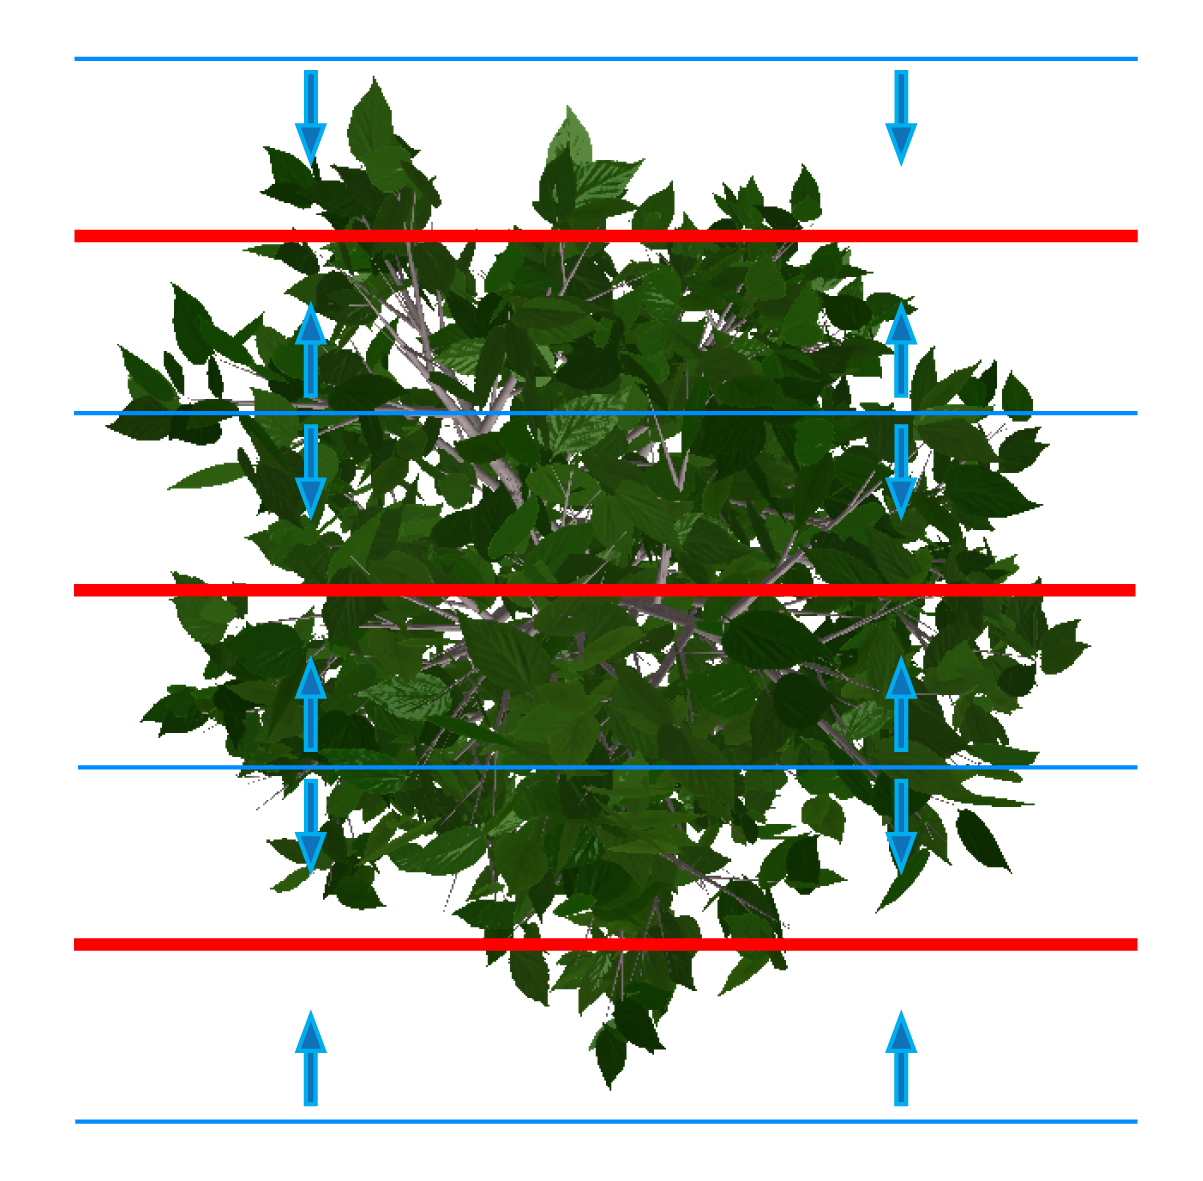
\includegraphics[width=0.5\textwidth]{./figures/slices.png}
\caption{ Tvorba řezů pro vícevrstvé billboardy. Jednotlivé textury řezů jsou znázorněny červeně. }
\end{center}
\label{fig:slicing}
\end{figure}
Čím je objekt od pozorovatele vzdálenější, tím méně se tyto efekty uplatňují a tím menší má objekt percepční váhu, proto lze v rámci zvýšení výkonu snižovat počet obrázků (textur) v trsu.
Protože se orientace trsu řezů vůči scéně nemění, mohou vznikat nepříjemné artefakty tím, že směr pohledu bude téměř rovnoběžný s rovinou některého z řezů. Z toho důvodu je dobré zajistit, aby se takové řezy vůbec nezobrazovaly.
Řezy lze předgenerovat pro statický strom a používat je následně pro každou instanci daného stromu ve scéně.


\subsection{Animace v image-base modelu}
\label{sec-ibAnimation}

Bohužel z povahy konstrukce trsu řezů dochází ke ztrátě velikého množství informací, které jsou podstatné pro provedení animace v rozsahu a kvalitě odpovídající postupu popsaného v kapitole Animace trojrozměrného modelu. Větve jsou například většinou zakryty listy. Jednotlivé listy se také překrývají a tak například o listech, které nejsou vidět nelze získat žádné informace. Naštěstí nemají modely zobrazené touto metodou vysokou percepční váhu (jde o nižší LOD) a lze si tudíž dovolit snížení kvality a přistoupit k animaci zcela jinak.
Základním předpokladem je, že deformace se provádí pouze v dvourozměrném prostoru textury jednoho řezu. Zatímco původní deformace je realizovatelná ve vertex shaderu, tento postup využije s výhodou možností fragment shaderu. Vyplývá z toho však nepříjemné omezení, které mění původní problém, který lze shrnout otázkou: \emph{„Kam se posune tento bod?“} (nazývejme {\bf přímá transformace}), na problém typu \emph{„Jaký bod se přesune do tohoto místa?“} (nazývejme {\bf zpětná transformace}). Fragment shader totiž neumožňuje měnit aktuálně zpracovávanému fragmentu pozici, na kterou bude zapsán ve výstupním bufferu. Uvážíme-li, že se na určitou pozici může po transformaci zobrazit i několik fragmentů, bylo by pro korektní zobrazení nutné projít každý texel textury provést přímou transformaci a zjistit, zda není dosaženo aktuální pozice. Takové řešení je ovšem značně nevhodné.

Jestliže je třeba provádět v rámci jediné textury různé transformace, které přísluší různým zobrazeným větvím, pak je třeba znát, jaká transformace se v daném bodě bude provádět. Musí být tedy předem jasné, jaká větev se do daného bodu může zobrazit. Současně s generováním textur pro jednotlivé řezy, je možné připravit i texturu, která bude tuto informaci obsahovat. Jednoduchým řešením, které lze i efektivně implementovat na GPU, je vytvoření oblastí, které odpovídají buňkám Voronoiova diagramu – tedy pro daný bod nalezneme nejbližší bod, kde je zobrazena větev ve výchozím stavu. Tento postup můžeme nazvat {\bf „propagace dat“}.

\begin{figure}[!hbt]
\label{fig:sliceBilboard}
\begin{center}
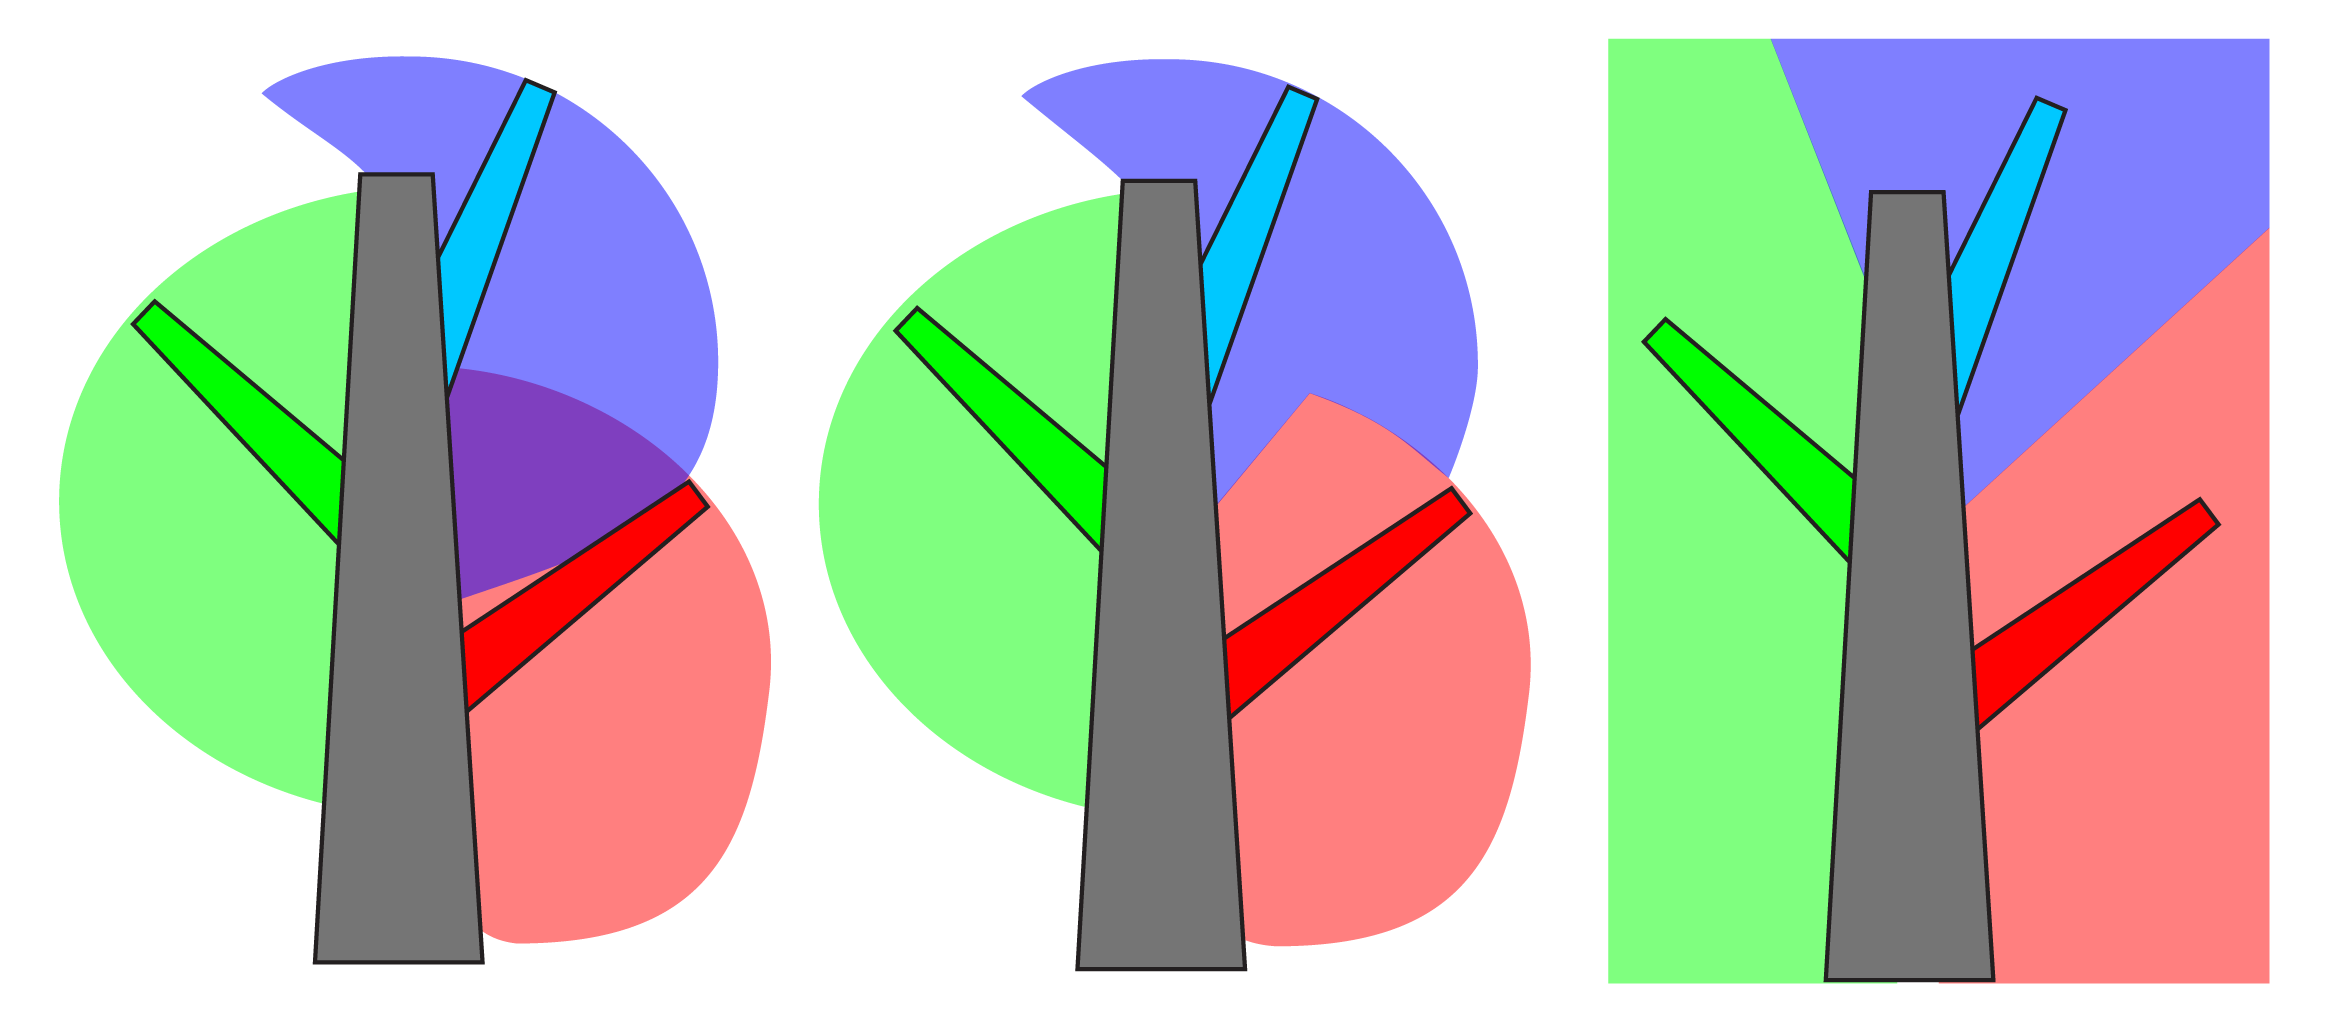
\includegraphics[width=0.75\textwidth]{./figures/dataExpansionPrinciple.png}
\caption[Schematicky znázorněné oblasti, kam se mohou větve deformovat]%
{Schematicky znázorněné oblasti, kam se mohou větve deformovat. Černě vytaženy obrysy výchozí polohy zobrazených větví
(vlevo) reálný ohyb – oblasti se překrývají, (uprostřed) oblasti bez překryvů, (vpravo) oblasti Voronoiova diagramu}
\end{center}
\end{figure}

Pokud tedy známe, jaká větev se může do daného bodu $P$ deformovat, známe také parametry této deformace. Z důvodů zachování koherence animace (větve se pohybují zhruba stejně) využijeme metodu deformace vycházející z ohybu trojrozměrného modelu. Trojrozměrný ohyb je prováděn v souřadném systému větve ($S_b$). Po převedení bázových vektorů ($\vec{r}_b$,$\vec{s}_b$,$\vec{t}_b$) do souřadného systému řezu ($S_p$ – tedy vektory $\vec{r}_p$,$\vec{s}_p$,$\vec{t}_p$) je možné postupovat prakticky stejně. Uplatníme myšlenkový model, kdy bod $P_0$ mimo větev (představovaná osou x) bude při deformaci udržovat svou relativní pozici na normále k větvi (viz obrázek \ref{fig:bendModel}). Potřebujeme tedy zjistit, ke kterému bodu větve je bod $P_p$ ukotven.

\begin{figure}[!hbt]
\begin{center}
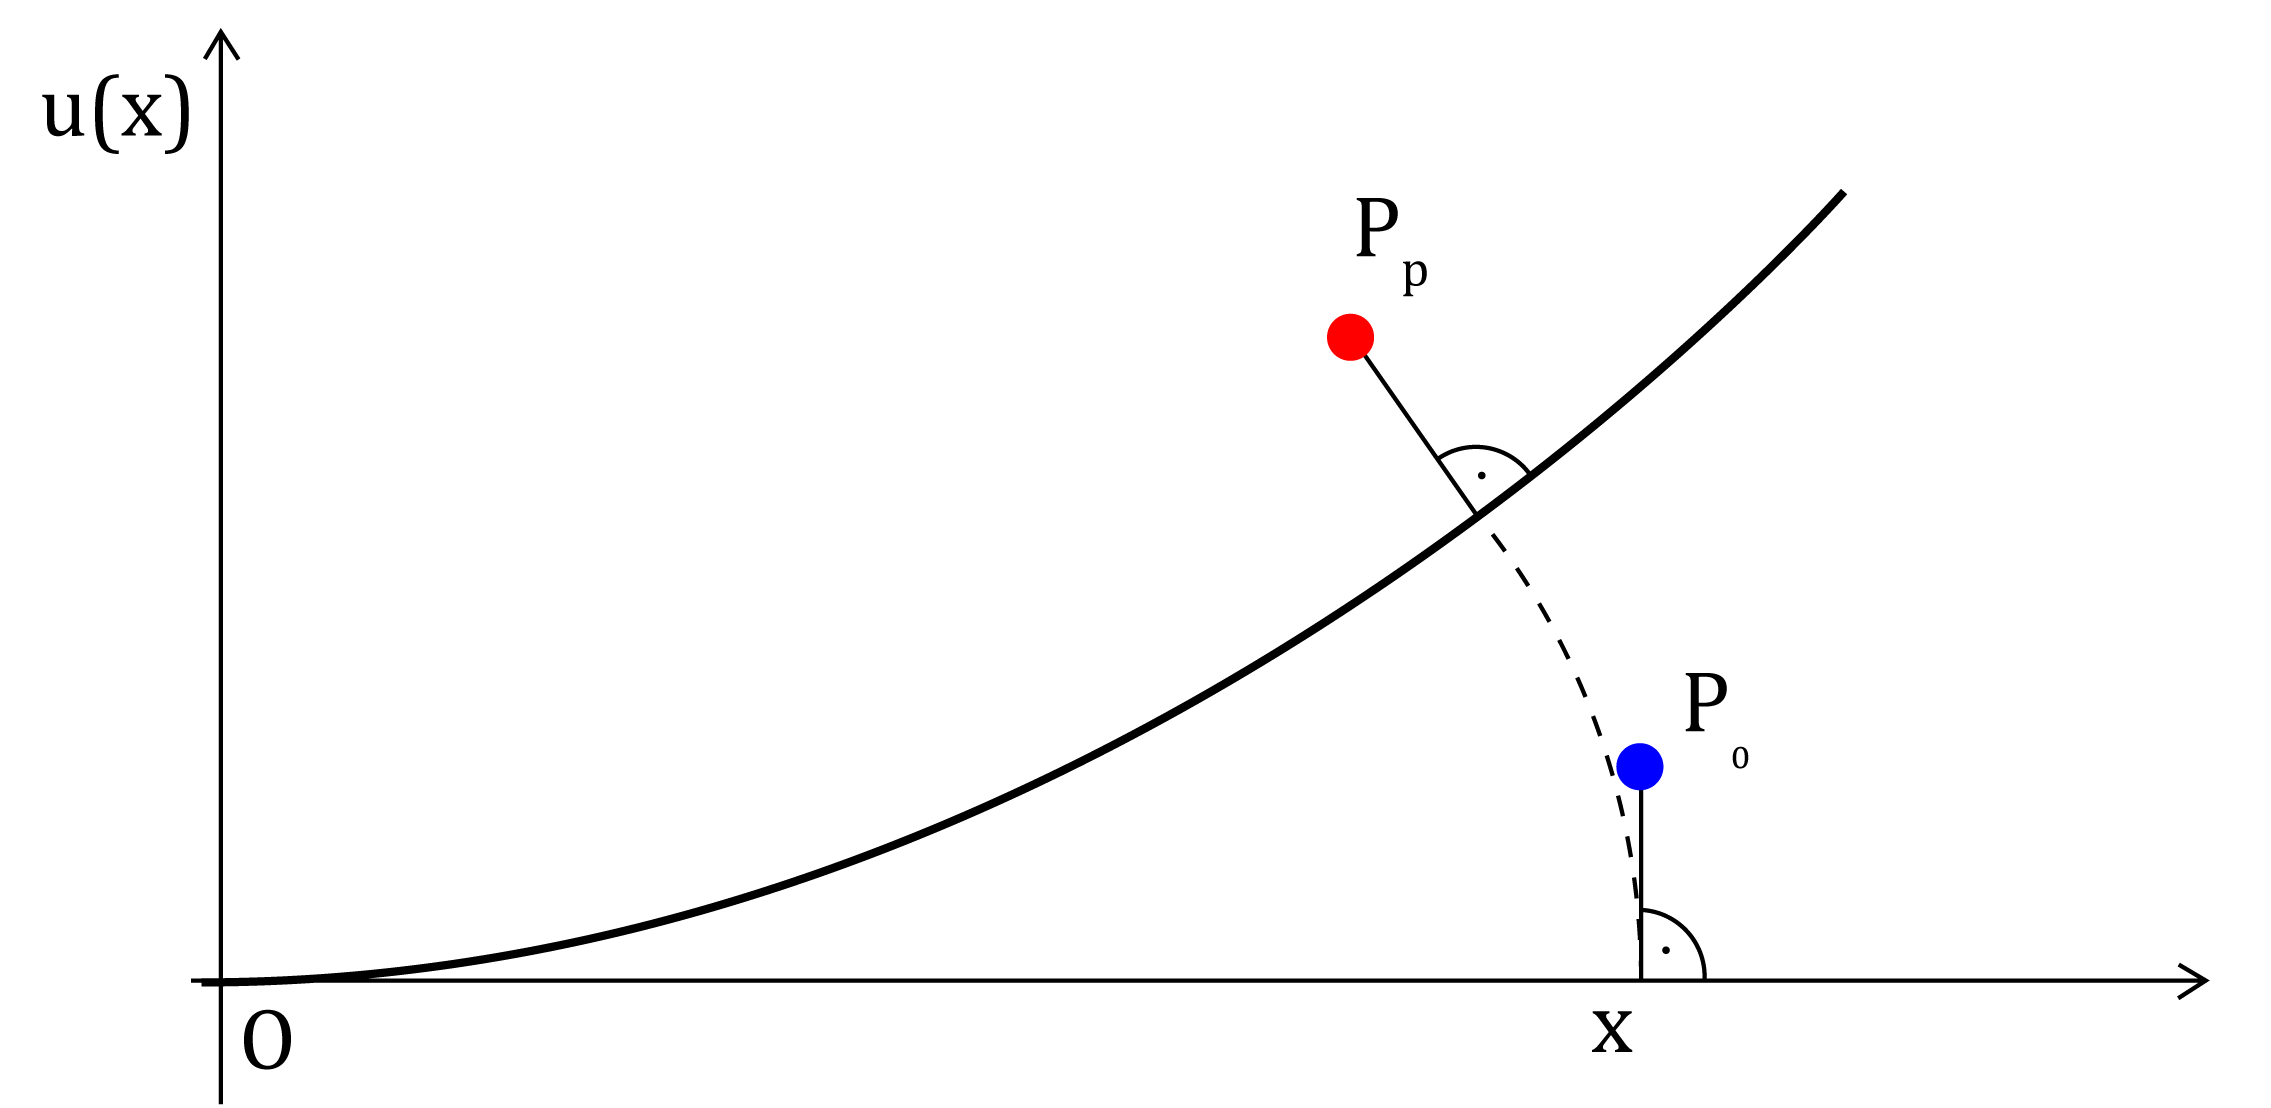
\includegraphics[width=0.5\textwidth]{./figures/revDef_ideal.png}
\caption{Myšlenkový model ohybu pomocí zpětné transformace\label{fig:bendModel}}
\end{center}
\end{figure}
 
Problém představuje určení parametru $x$ ohybové funkce $u(x)$ pro bod $P_p$ (deformovaný z $P_0$), který zmíněnou polohu na větvi definuje. Pro přesné určení je nutné zjistit nejbližší bod na ohybové funkci a pro ten pak zjistit jeho vzdálenost na křivce od počátku. 
\begin{figure}[!hbt]
\begin{center}
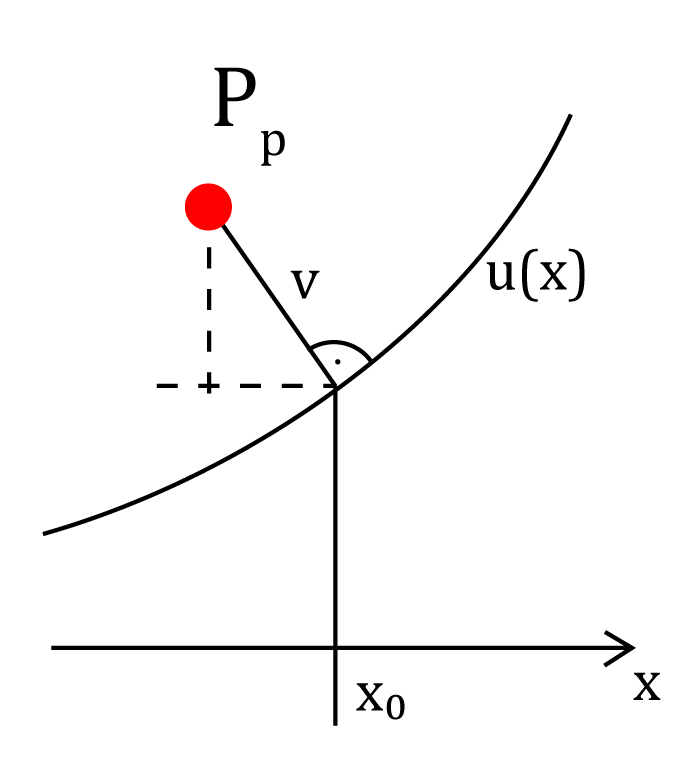
\includegraphics[width=0.25\textwidth]{./figures/revDef_dist.png}
\caption{Zjišťování nejbližšího bodu na ohybové křivce $u(x)$\label{fig:closestPointOnCurve}}
\end{center}
\end{figure}

Bod $x_0$ lze určit z následujících rovnic, kde hledáme minimum pro vzdálenost $v$:

\begin{align}
\frac{\mathrm {d}{v}}{\mathrm {d}{x_0}} &= 0 \nonumber\\
v &= \sqrt{(x_0 - P_{px})^2 + (u(x_0) - P_{py})^2} \nonumber\\
\frac{\mathrm {d} \sqrt{(x_0 - P_{px})^2 + (c_2x_0^2 +c_4x_0^4 - P_{py})^2}}{\mathrm{d}x_0} &=0
\end{align}
Řešení je omezeno podmínkou:
\begin{align}
P_{px} \neq \pm \sqrt {\frac{-c_2 \pm \sqrt{c_2^2 - 4c_4P_{py}}}{2c_4}}
\end{align}

a transformuje se na problém hledání kořenů polynomu 7. stupně:

\begin{align}
\label{closestPointEq}
4c_4^2 x^7 + 6c_2c_4x^5 + (2c_2^2 - 4P_{py}c_4)x^3 + (1-2P_{py}c_2)x - P_{px} &= 0
\end{align}

Tento polynom nemá triviální řešení a může se stát, že řešení je i několik – což odpovídá situaci, kdy se více bodů z křivky deformuje do stejného místa (viz obrázek ~\ref{fig:multisolution} ).
\begin{figure}[!hbt]
\begin{center}
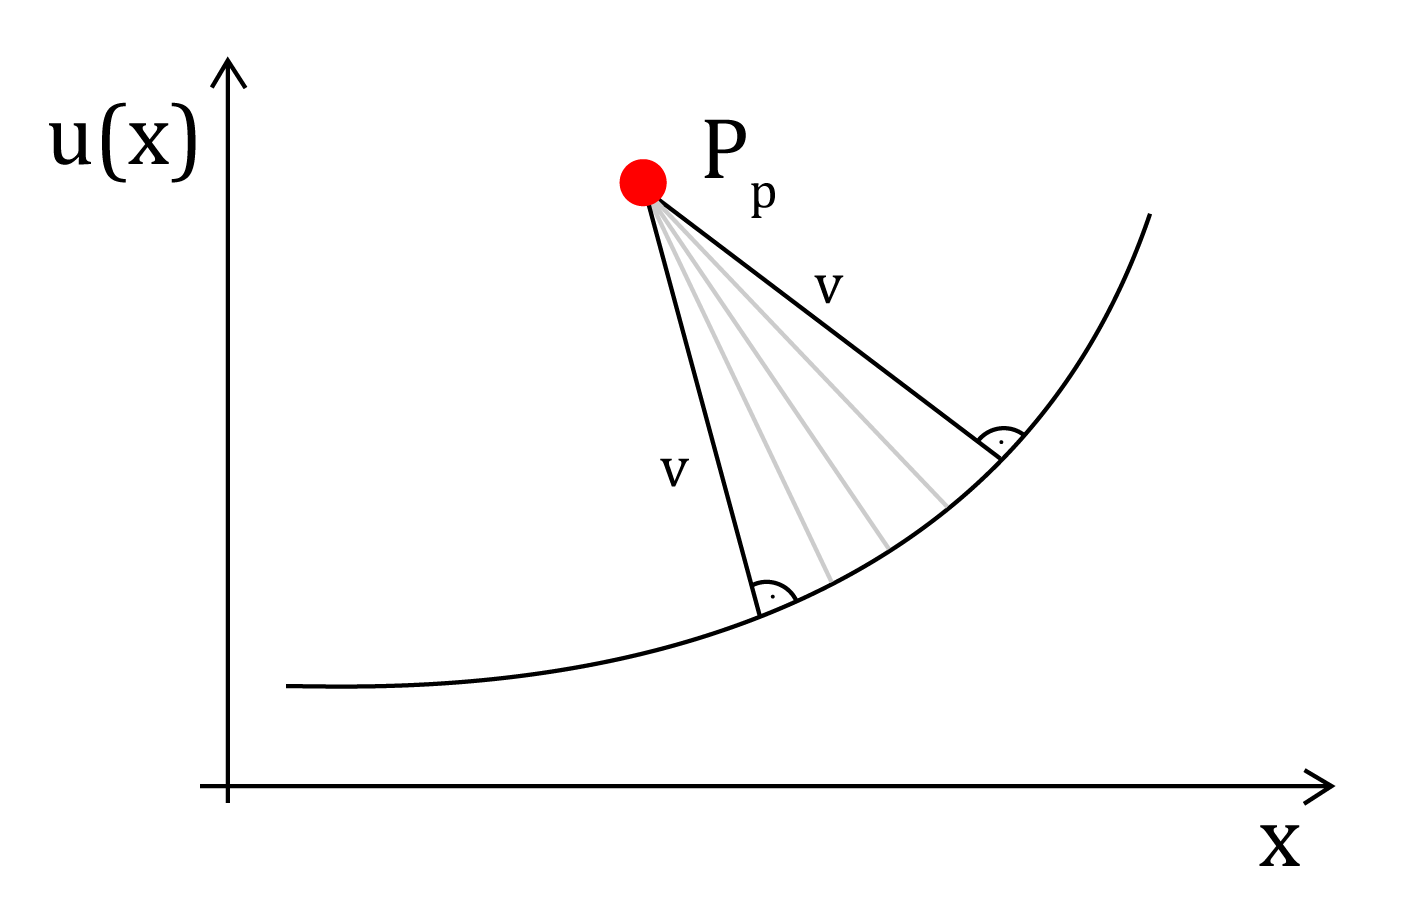
\includegraphics[width=0.5\textwidth]{./figures/revDef_multisolution.png}
\caption[Mnohoznačnost při zpětné transformaci]
{Znázornění problému mnohoznačnosti při určování, který bod je řídící pro zpětnou deformaci bodu $P_p$. U reálného stromu dojde v tomto případě ke kolizi takových větví.\label{fig:multisolution}}
\end{center}
\end{figure}

Krom obtíží s řešením kořenů polynomu \eqref{closestPointEq} se tak přidává i určitá nejednoznačnost. Stále je však ještě potřeba vyřešit vzdálenost takto nalezeného bodu na ohybové křivce. Uvážíme-li, že takový složitý postup by se měl provádět pro každý zobrazovaný fragment textury, dostaneme se do patové situace.
Zde je třeba rezignovat na dodržení shodného postupu jako v případě přímé deformace geometrie. Počáteční bod $O$ příslušné větve převedeme do souřadného systému textury ${S_p}$ a zjistíme projektovanou délku $L$ větve. {\bf Hledanou hodnotu x pak nahradíme vzdáleností $\left| OP \right|$, kterou normujeme délkou $L $ a omezíme na rozsah $\left \langle 0;1 \right \rangle$ }. Pro takovou hodnotu $x$ určíme deformační vektor $\vec{d}$ (posunutí bodu) a aplikujeme v opačném směru $\vec{-d}$ než při přímé transformaci.
 
\begin{figure}[!hbt]
\begin{center}
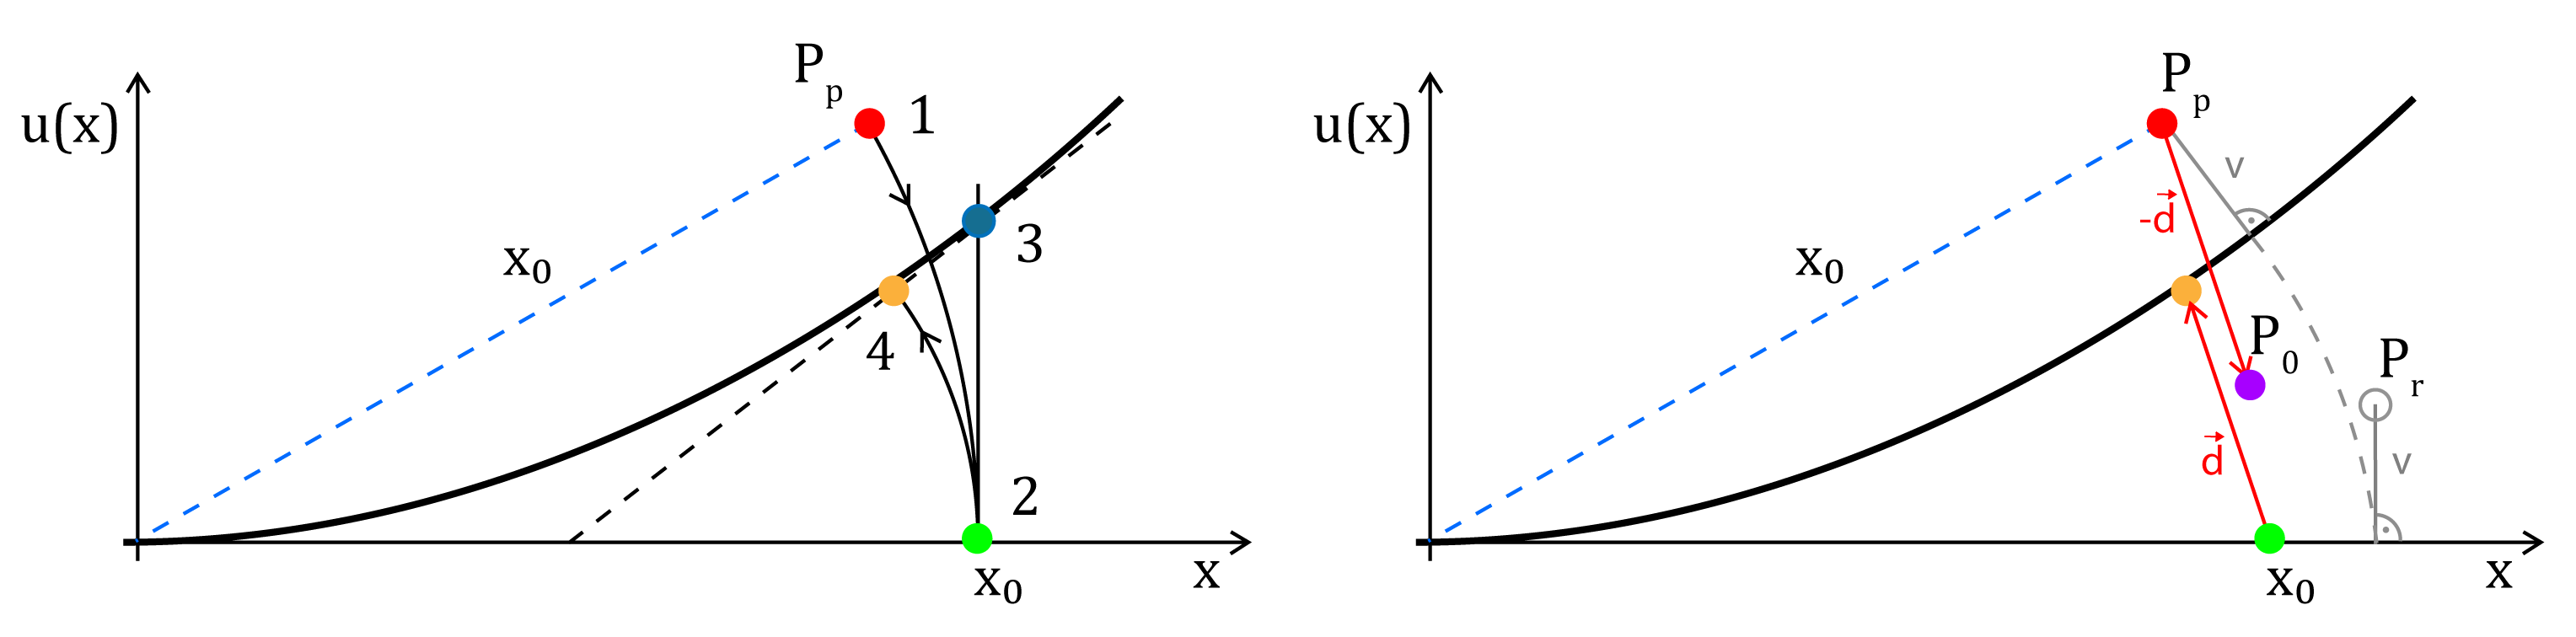
\includegraphics[width=1.0\textwidth]{./figures/revDef_process.png}
\caption[Postup zpětné transformace]
{Postup zpětné transformace: (vlevo) – postup určení deformace: Bod $P_p$ (1), pro který určujeme deformaci je ve vzdálenosti $x_0$ od počátku (2). Zjistíme hodnotu ohybové funkce v bodě $x_0$ (3). Provedeme korekci délky (4).
(vpravo) – určíme vektor posunutí $\vec{d}$ mezi body $x_0$ a (4) (v obrázku vlevo) odečtením od bodu $P_p$ se dostáváme na pozici předobrazu $P_0$. Šedivě je naznačen bod $P_r$, jež je skutečným předobrazem respektujeme-li myšlenkový model. \label{fig:backwardTransformationProcess}}
\end{center}
\end{figure}
\pagebreak
Je patrné, že chyba způsobená takovou hrubou aproximací $x_0$ je relativně malá pro body $P_p$, ležící přímo na ohybové křivce, ale roste tím víc, čím je od ní bod vzdálenější. Použitím vztahů \eqref{lengthCorrection} aplikovaným na projektované bázové vektory $\vec{r}_p$, $\vec{s}_p$ (zastoupené vektorem $\vec{b}_p$) dostaneme upravené vztahy pro korekce délky $\vec{c}_{\vec{b}}$, $\vec{c}_{\vec{b}}$.

\begin{align} 
\vec{c}_{\vec{b} }&= \vec{t} + \vec{b} \cdot f'_{\vec{b} } (x)\cdot\frac {d_{\vec{b} }(x)}{s_{\vec{b} }(x)}
 \end{align}

Deformaci v prostoru textury lze tedy popsat následovně:

\begin{align}
\label{backwardDeformation} 
\vec{P}_0 &= \vec{P}_p - \left ( u_{\vec{r}} (x) \cdot \vec{r}_p + u_{\vec{s}} (x) \cdot \vec{s}_p - \left (\vec{c}_{\vec{r}} +\vec{c}_{\vec{s}}  \right ) \right )
\end{align}


Zpětnou deformaci lze provádět i hierarchicky a to v pořadí od nejnižší úrovně větví v hierarchii až po kmen (tedy opačně, než v přímé transformaci). Je však nutné vyvážit náročnost takového postupu a jeho přidanou hodnotu. Například je možné deformaci provádět pro několik nejvyšších úrovní hierarchie. 
S opačným postupem tvorby hierarchické deformace v image-based modelu souvisí i problém správné aplikace směrové složky větru. Ve vztahu \eqref{windEq} je použit vektor $\vec{t}$ ovlivněný nadřazenými deformacemi. Ten však při opačném postupu zpětné deformace není znám. Předpokládáme-li provádění zpětné deformace pouze ve dvou úrovních (kmen + větve první úrovně) a rozumě malé výchylky, pak lze za vektor $\vec{t}$ dosadit nedeformovaný vektor $\vec{t}_p$, místo $\vec{W}$ použijeme $\vec{W}_p$ (směr větru v souřadné soustavě řezu). Vzniklá chyba není natolik vážná, aby představovala překážku u modelů s nižší percepční vahou, jakými nižší stupně LOD bezpochyby jsou.

Popsaná metoda má předpoklad dobře fungovat pro větve tvořící siluetu stromu v daném řezu. U takových větví se předpokládá, že jejich podélný vektor je zhruba rovnoběžný s rovinou řezu. Současně je třeba si uvědomit, že i fáze propagace dat má určitá omezení a funguje lépe pro siluetové větve. Jak se však ukazuje, právě tyto větve hrají největší roli při pozorování stromu s nižší percepční vahou. Hrají i podstatnou roli při přechodu mezi úrovněmi LOD.

Zbývá vyřešit pohyb jednotlivých listů. Pohybem větví nižších úrovní hierarchie a listů vzniká vysokofrekvenční šum v prostoru obrazu. Tento šum pozorovatel vnímá, ale nerozeznává již, jestli je způsoben pohybem větví, či samotných listů. Lze ho tedy napodobit použitím jediné deformace. Pro šum vyšších frekvencí je zároveň těžké rozlišit, zda jde čistě o pohyb, či jen změny barvy. Představíme-li si například, že list je zobrazen do jediného pixelu, pak pouhým natáčením listu zjevně měníme barvu zmíněného pixelu (barevný šum). Nerotační pohyb listu může způsobit obarvení jiného pixelu (pohybový šum). Pohyb listů může pak ústit v určité nepravidelné chvění elementárních fragmentů obrazu (případně větších oblastí – podle toho, kolik fragmentů zobrazuje stejný list).
Pohybovou složku šumu lze vcelku dobře napodobit metodou zvanou {\bf displacement-mapping}. V základní verzi získává z řídící textury informace o posunutí v prostoru deformovaného obrazu – v tomto případě barevné textury. Vhodnými změnami řídící textury (posun souřadnic, kombinace různých textur) lze plynule deformovat výsledný obraz. 
\begin{figure}[!hbt]
\begin{center}
$\begin{array}{cc}
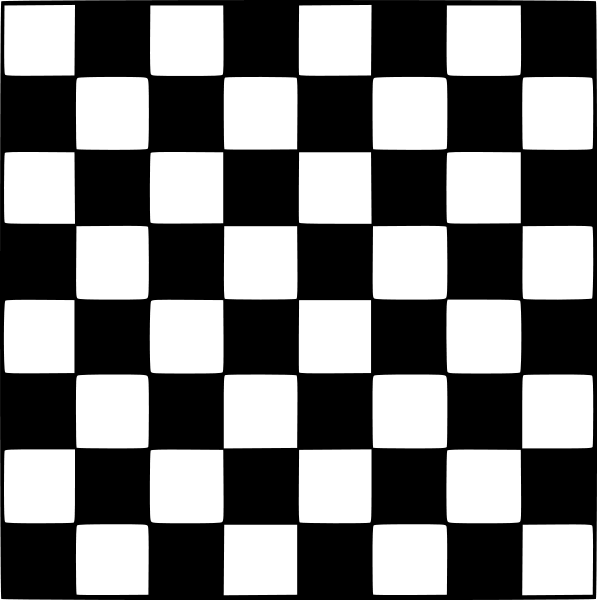
\includegraphics[width=0.35\textwidth]{./figures/distortion_before.png}&
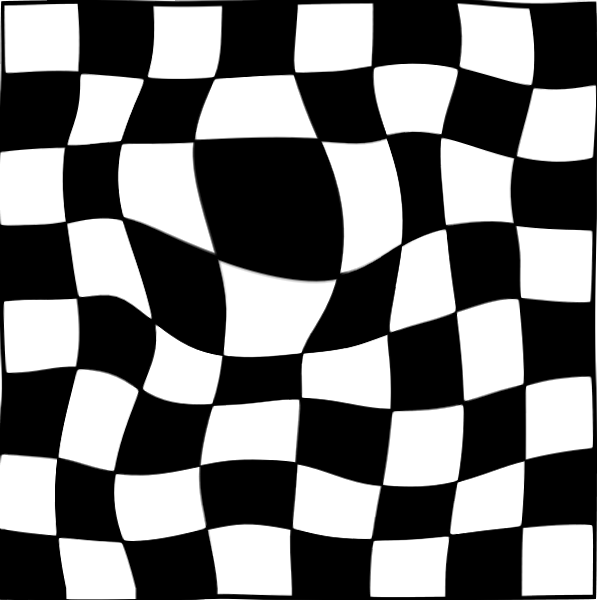
\includegraphics[width=0.35\textwidth]{./figures/distortion_after.png}
\end{array}$
\caption[Postup zpětné transformace]
{Postup zpětné transformace: (vlevo) – postup určení deformace: Bod $P_p$ (1), pro který určujeme deformaci je ve vzdálenosti $x_0$ od počátku (2). Zjistíme hodnotu ohybové funkce v bodě $x_0$ (3). Provedeme korekci délky (4).
(vpravo) – určíme vektor posunutí $\vec{d}$ mezi body $x_0$ a (4) (v obrázku vlevo) odečtením od bodu $P_p$ se dostáváme na pozici předobrazu $P_0$. Šedivě je naznačen bod $P_r$, jež je skutečným předobrazem respektujeme-li myšlenkový model. \label{fig:backwardTransformationProcess}}
\end{center}
\end{figure}


Šumový displacement-mapping je možné zapsat například takto:

\begin{align} 
color &= T_{color}(T_{def}(\vec{o}_t + t \cdot \vec{d}_1)+T_{def}(\vec{o}_t + t \cdot \vec{d}_2)),
\end{align}
kde $T_{def}(\vec{x})$ je texturovací funkce, jež zobrazuje souřadnice $\vec{x}$ na jiné, a $T_{color}(\vec{x})$ přiřazuje daným souřadnicím $\vec{x}$ barvu. 
Barevnou složku šumu je možné vytvořit například tak, že pro každý zobrazený list v řezu měníme jeho natočení ke světlu (normálu) a následně provádíme standardní vyhodnocení Phongova osvětlovacího modelu.

\pagebreak
\subsection{Řízení úrovně detailu}
\label{sec-LODcontrol}
V předchozích kapitolách jsou navrženy metody, jak zobrazovat vegetaci (stromy) ve třech různých stupních detailu. Nejvyšší (označme ji \emph{LOD\_0}) využívá podrobné geometrické reprezentace a poskytuje nejlepší kvalitu zobrazení pro pohledy zblízka. Přesvědčivě tak lze zobrazit i jednotlivé pohybující se listy stromu. LOD\_0 je však vcelku náročná na výkon a není možné ji uplatnit plošně na všechny stromy rozsáhlé lesní scény. Pro stromy s nižší percepční vahou (není třeba je zobrazovat tak podrobně) byly navrženy image-based metody (označme LOD\_1 a LOD\_2). Ty poskytují sice nižší kvalitu zobrazení (na úrovni zobrazení a pohybu celého stromu), ale jsou méně náročné na výkon. 
\begin{figure}[!hbt]
\begin{center}
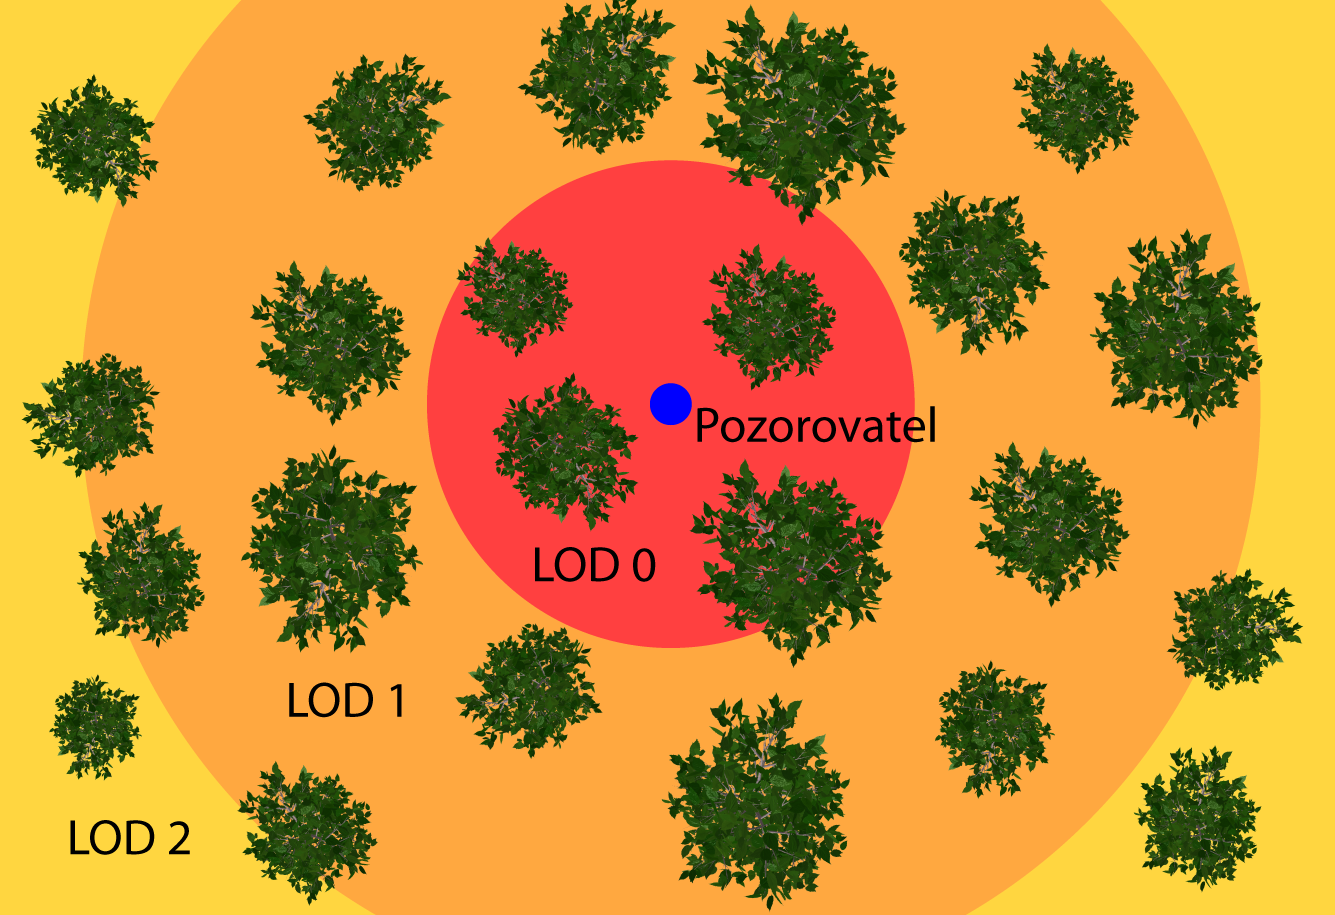
\includegraphics[width=0.75\textwidth]{./figures/LODcontrol.png}
\caption{Znázornění zón, kde se instance stromů vykreslují danou metodou.\label{fig:lodZones}}
\end{center}
\end{figure}

Pro určení přibližné percepční váhy se běžně využívá vzdálenostní kritérium. Blízké stromy v okolí pozorovatele jsou tedy zobrazeny metodou LOD\_0, od určité vzdálenosti $v_1$ se využívá metody LOD\_1 a obdobně pro vzdálenost $v_2$ a metodu LOD\_2, přičemž platí, že $0<v_1<v_2$ .

Jedná se tedy o diskrétní třístupňový LOD systém. Určení vzdálenosti k jednotlivým instancím stromu lze provádět buď v prostoru (vhodné např. aplikace typu letecký simulátor), nebo pouze v horizontální rovině (aplikace s pohledem omezeným na pohled z okolí úrovně terénu). Vzdálenosti $v_1$ a $v_2$ je třeba přizpůsobit konkrétním modelům vegetace a scéně obecně, stejně jako optimalizaci z hlediska výkonu, na který mají podstatný vliv.


\subsection{Přechody mezi úrovněmi detailu}
\label{sec-LODtransitions}
